% ============================================================
% Privacy-Preserving Load Forecasting and Energy Optimization
% in IoT-Enabled Smart Homes
% IEEE Journal Template (IEEEtran)
% ============================================================
% Instructions:
%   1. Run: python results/generate_graphs.py
%   2. Upload this .tex file + all PDFs from results/graphs/ to Overleaf
%   3. Place graph PDFs in a subfolder called "graphs/" on Overleaf
%   4. Compile with pdfLaTeX
% ============================================================

\documentclass[journal]{IEEEtran}

% *** GRAPHICS RELATED PACKAGES ***
\ifCLASSINFOpdf
  \usepackage[pdftex]{graphicx}
  \graphicspath{{graphs/}}
  \DeclareGraphicsExtensions{.pdf,.jpeg,.png}
\else
  \usepackage[dvips]{graphicx}
  \graphicspath{{graphs/}}
  \DeclareGraphicsExtensions{.eps}
\fi

% *** MATH PACKAGES ***
\usepackage{amsmath,amssymb,amsfonts}

% *** CITATION PACKAGES ***
\usepackage{cite}

% *** TABLE PACKAGES ***
\usepackage{booktabs}
\usepackage{multirow}

% *** FLOAT PACKAGES ***
\usepackage{float}

% *** URL PACKAGES ***
\usepackage{url}

% Indian Rupee symbol
\newcommand{\rupmark}{\text{\small\textrm{\textup{INR}}}}

% correct bad hyphenation here
\hyphenation{fed-er-ated Stack-el-berg pri-va-cy op-ti-mi-za-tion}

\begin{document}

\title{Privacy-Preserving Load Forecasting and Energy Optimization in IoT-Enabled Smart Homes Using Federated Learning and Game-Theoretic Scheduling}

\author{Shresht~Kumar~Linga~(24BCE5508)
        and~Marun~VP~(24BCE5544)% <-this % stops a space
}

%\markboth{IEEE Journal,~Vol.~XX, No.~X, March~2026}%
%{Linga \MakeLowercase{\textit{et al.}}: Privacy-Preserving Load Forecasting in IoT-Enabled Smart Homes}

\maketitle

% ============================================================
%                        ABSTRACT
% ============================================================
\begin{abstract}
The proliferation of Internet-of-Things (IoT) devices in smart homes has accelerated the deployment of advanced energy management systems capable of monitoring and controlling residential electricity consumption in real time. However, the dual imperatives of accurate demand forecasting and appliance schedule optimization remain fundamentally constrained by conflicting requirements: centralized learning approaches that enable high-accuracy predictions inherently risk exposing sensitive consumer behavioral data, while decentralized methods often sacrifice forecasting precision and lack economically informed cost signals. Existing solutions, including static Time-of-Use (TOU) pricing, independent deep reinforcement learning agents, and conventional federated frameworks, address these challenges in isolation, failing to jointly optimize privacy, forecast accuracy, grid stability, and user comfort under a unified and physically constrained architecture.

This paper presents a six-stage hybrid intelligent framework that integrates a Digital Twin Simulator for high-fidelity synthetic data generation, a $\beta$-Variational Autoencoder ($\beta$-VAE, $\beta = 0.5$) for nonlinear dimensionality reduction, a Federated Gated Recurrent Unit (FedGRU) network for distributed privacy-preserving load forecasting, a Hierarchical Stackelberg Game for demand-responsive dynamic pricing, a Differential Evolution (DE/rand/1/bin) optimizer with an eight-term multi-objective fitness function for constrained appliance scheduling, and an interactive visualization dashboard. The framework operates end-to-end on raw IoT data without exposing individual consumption records, enforcing data locality through the FedAvg protocol across 50 distributed smart home clients.

Experimental evaluation on a synthetic dataset of 144,000 records spanning 50 homes over 30 days demonstrates that the proposed framework achieves a 46.2\% daily energy cost reduction (from 1308\,INR to 704\,INR), a 23.0\% peak load reduction, and robust forecasting accuracy with a Mean Absolute Error of 1.846\,kW and Root Mean Square Error of 2.502\,kW after 20 federated communication rounds. Comparative analysis against three recent IEEE baselines confirms balanced superiority across all evaluation dimensions.
\end{abstract}

% ============================================================
%                     INDEX TERMS
% ============================================================
\begin{IEEEkeywords}
Federated Learning, Smart Home Energy Management, Variational Autoencoder, Stackelberg Game, Differential Evolution, Privacy-Preserving IoT
\end{IEEEkeywords}

\IEEEpeerreviewmaketitle

% ############################################################
%              SECTION I: INTRODUCTION
% ############################################################
\section{Introduction}

The rapid proliferation of Internet-of-Things (IoT) architectures has transformed traditional residential grids into smart homes, forming the foundational bedrock of modern smart cities \cite{alzamil2025federated, alfaverh2020demand}. At the heart of this transformation lies the fundamental challenge of energy optimization, which seeks to dynamically balance electricity demand with variable supply without compromising end-user comfort \cite{zhang2025demand}. Driven by the widespread deployment of advanced metering infrastructure (AMI) and highly controllable smart appliances, residential load forecasting has emerged as a critical subdomain \cite{wang2025multi-gradient-descent}. Accurate, high-resolution forecasting enables grid operators to execute proactive energy management strategies and implement dynamic pricing mechanisms that incentivize peak-load reduction. Consequently, smart home energy optimization now strictly depends on the tight coupling of data-driven demand prediction and computationally robust scheduling algorithms \cite{aguiar2021network-constrained}.

Despite the conceptual promise of smart home energy management, the problem statement is inherently characterized by conflicting physical and sociological constraints: attempting to achieve high-accuracy demand predictions inevitably demands extensive aggregation of granular, appliance-level consumption data, which fundamentally risks consumer privacy \cite{fan2025adaptive, wang2024blockchain-based}. High-frequency power signatures can inadvertently expose sensitive behavioral patterns, occupancy states, and socioeconomic markers to malicious actors or untrusted central servers. This privacy loss critically hampers the widespread adoption of automated demand response programs \cite{balint2023using}. The socio-technical impact of solving this multidimensional problem is vast---developing localized, secure, and economically viable optimization paradigms is mandatory to curb the escalating peak energy demands, reduce greenhouse gas emissions, and lower utility bills in the residential sector \cite{dong2020energy, bahrami2021deep}.

Existing energy management and forecasting systems exhibit critical limitations when addressing these interdependent challenges. Centralized deep learning frameworks, while analytically sound, mandate the massive transmission of raw household IoT data to a cloud server, creating unacceptable singular points of failure and explicit privacy violations \cite{wang2024blockchain-based, fan2025adaptive}. Conversely, purely decentralized independent agents tend to lack economic coordination, typically ignoring broader grid-capacity constraints and failing to react synergistically to dynamic pricing signals \cite{lee2018light-weight}. Furthermore, systems that independently address either forecasting or scheduling frequently drop the physical coupling between them; naive schedules fail to adapt when demand abruptly peaks due to unforeseen thermal loads \cite{huang2019demand, zhang2025demand}.

To resolve this severe dichotomy, advanced privacy-preserving algorithms and complex metaheuristic optimizers play a defining role. Federated learning serves as a mathematically rigorous paradigm for distributed model training, effectively decoupling analytical power from raw data aggregation by ensuring that sensitive records never leave local physical boundaries \cite{mao2023communication-efficient, danish2025block-fedl:}. In parallel, sophisticated game-theoretic models, particularly non-cooperative hierarchical formalisms, inject critical economic rationality into the network, dynamically aligning end-user optimization goals with overarching utility constraints \cite{dong2020energy}. Lastly, evolutionary computation serves as the algorithmic engine uniquely capable of unspooling the rugged, discontinuous multi-objective fitness landscapes governed by complex home thermal dynamics and discrete appliance activation states \cite{zhang2025aggregator-grid}.

In this paper, we propose a comprehensive hybrid intelligent system engineered to jointly optimize privacy-preserving load forecasting and discrete energy scheduling within IoT-enabled smart homes. The framework securely forecasts residential demand via a Federated Gated Recurrent Unit (FedGRU) network operating strictly on compressed $\beta$-Variational Autoencoder ($\beta$-VAE) latent representations, neutralizing data leakage risks at the edge. The securely aggregated load predictions subsequently drive a Hierarchical Stackelberg pricing game, establishing an equilibrium that balances grid capacity with consumer utility. Finally, a specialized Differential Evolution (DE) optimizer evaluates candidate appliance schedules against an intricate multi-objective fitness function to generate mathematically constrained, cost-effective activation plans.

The specific unique contributions of this work are highlighted as follows:
\begin{itemize}
    \item We formulate an interconnected pipeline where $\beta$-VAE non-linear dimensionality reduction and Federated GRU algorithms are pipelined, enabling accurate time-series forecasting while strictly bounding the communication payload and guaranteeing absolute raw data privacy across remote IoT nodes.
    \item We design a dynamic Hierarchical Stackelberg game tightly integrated with federated forecasting outputs, creating a closed-loop demand response market model that dynamically computes equilibrium electricity pricing.
    \item We introduce a highly constrained multi-objective Differential Evolution (DE/rand/1/bin) optimizer evaluating an eight-term custom fitness function to simultaneously execute exact peak-shaving, thermal comfort preservation, and physical constraint adherence.
    \item We develop a high-fidelity Digital Twin Simulator simulating stochastic Markov-based human occupancy and complex thermal dynamics, explicitly tailored to generate massive, realistic datasets to robustly benchmark the proposed joint-optimization workflow.
\end{itemize}

The remainder of this paper is structured as follows: Section II provides a comprehensive review of related works and delineates the existing research gaps. Section III presents an overview of the proposed system architecture. Section IV rigorously details the mathematical formulations and implementations of the six core system modules. Section V discusses the dataset, experimental validation, and quantitative comparative analysis. Finally, Section VI concludes the paper and outlines future research trajectories.

% ############################################################
%              SECTION II: RELATED WORKS
% ############################################################
\section{Related Works}

The problem of smart home energy management, demand forecasting, and privacy-preserving automation has garnered significant attention from the industrial informatics and computational intelligence communities. In recent years, researchers have conceptualized various distinct approaches ranging from reinforcement learning to spatiotemporal federated setups, each mitigating aspects of this multiobjective domain \cite{rahman2025electrical, zhang2025adaptive}. This section critically reviews recent literature (2018--2025) across key algorithmic domains.

Researchers investigating deep reinforcement learning (DRL) have actively explored algorithmic adaptations to control appliance states under real-time conditions. Notably, Li \textit{et al.} \cite{madrl2025} developed a massive multi-agent DRL framework combining Q-learning agents to handle dynamic pricing, validating their architecture via substantial cost-to-comfort improvements. Similarly, Bahrami \textit{et al.} \cite{bahrami2021deep} and Tang \textit{et al.} \cite{tang2024dynamic} introduced demand response coordination models utilizing deep reinforcement learning to coordinate dynamic competitive interactions for demand response, optimizing continuous action domains. While these DRL systems iteratively solve for comfort optimization, they generally mandate enormous, centralized experience replay buffers and lack the long-term temporal lookahead inherent in seq2seq forecasting models, often failing when operating outside their trained distributional environments. 

Conversely, the necessity for robust forecasting models decoupled from privacy infringement has recently accelerated the integration of Federated Learning (FL) inside smart grids. Wang \textit{et al.} \cite{stfl2025} pioneered a spatiotemporal federated framework for privacy-preserving load forecasting, employing clustering strategies to bypass data centralization. In tandem, Alzamil \textit{et al.} \cite{alzamil2025federated} successfully validated federated deep learning for processing non-i.i.d sequential prediction tasks physically located un-aggregated at IoT endpoints. Furthermore, Wang \textit{et al.} \cite{wang2025multi-gradient-descent} proposed multi-gradient-descent collaborative learning functions, driving a parity-oriented formulation that tailored the aggregated global weights to individual consumer dynamics. Notably, Mao \textit{et al.} \cite{mao2023communication-efficient} introduced communication-efficient updates, drastically mitigating network latency during energy management epochs. Additionally, Wu \textit{et al.} \cite{wu2025privacy} engineered asynchronous protocols for edge-based energy scheduling, while Sharma \textit{et al.} \cite{sharma2024decentralized} extended these principles strictly to decentralized demand response. However, these FL frameworks overwhelmingly solve prediction challenges in pure isolation, entirely omitting necessary real-world market-responsive pricing dynamics and physically bound appliance control execution. To manage localized noise and dimensionality burdens prior to federated transmission, Fan \textit{et al.} \cite{fan2025adaptive} effectively demonstrated adaptive methods against stochastic noise injection inside real grid distributions.

In parallel with learning-oriented methods, game-theoretic economic models and metaheuristic operations have been optimized to regulate electricity markets and combinatorial scheduling. Aguiar \textit{et al.} \cite{aguiar2021network-constrained} addressed non-cooperative supply-demand alignment utilizing a Stackelberg game approach, successfully limiting macroscopic grid peak fluctuations. Dong \textit{et al.} \cite{dong2020energy} subsequently bridged game theory with consumer management by optimizing Nash equilibrium states against cost using hierarchical strategies. Additionally, optimization systems like the Big Data-Intelligence Analytics (BDIA) framework by Zheng \textit{et al.} \cite{bdia2025} mapped IoT appliance behavior against static pricing models using massive computational analytics. To manage complex constraint bounds in load scheduling, Zhang \textit{et al.} \cite{zhang2025aggregator-grid} applied adaptive algorithms respectively to penalize infeasible load curves and optimize combinatorial tasks precisely. Decentralized structures leveraging blockchain layers have also emerged, with Danish \textit{et al.} \cite{danish2025block-fedl:} verifying distributed smart home control ledgers that resist tampering.

Despite substantial advancements in these distinct verticals, a significant research gap persists: a distinct lack of physical integration between secure, non-linear load forecasting mechanisms and multi-user game-theoretic scheduling platforms within a single deterministic boundary. Most federated systems, such as STFL, halt computational effort at the prediction horizon, failing to implement any post-forecast schedule optimizers. Simultaneously, optimization frameworks, such as BDIA and MADRL, implicitly assume fully static or external price structures. The proposed system distinctively addresses these severe limitations by architecting a completely unbroken sequence. By binding a $\beta$-VAE filtered FedGRU prediction network to a continuous Hierarchical Stackelberg game, our model automatically determines a real-time reactive electricity price. The DE optimizer subsequently intercepts this newly formulated price signal to solve an eight-dimensional constraint framework, ensuring that the final appliance schedules reflect actual predictive intelligence, optimal grid capacity balances, and rigorous personal data secrecy simultaneously.

% ############################################################
%              SECTION III: PROPOSED SYSTEM
% ############################################################
\section{Proposed System}

\subsection{Overview}

The proposed framework addresses three fundamental challenges in smart home energy management: (1) accurate load forecasting under data privacy constraints, (2) economically rational dynamic pricing in multi-user networks, and (3) multi-objective appliance schedule optimization under physical constraints. To tackle these challenges simultaneously, we present a six-stage hybrid intelligent system that integrates a Digital Twin Simulator for synthetic data generation, a $\beta$-Variational Autoencoder ($\beta$-VAE) for latent feature extraction, a Federated Learning-based Gated Recurrent Unit (FedGRU) network for privacy-preserving load forecasting, a Hierarchical Stackelberg Game for dynamic electricity pricing, a Differential Evolution (DE) optimizer for constrained schedule optimization, and an interactive visualization dashboard.

The key innovation lies in the end-to-end integration of these components into a unified pipeline where each module feeds into the next: the Digital Twin generates realistic training data, the $\beta$-VAE compresses high-dimensional IoT features into compact latent representations, the FedGRU uses these representations to forecast future demand without exposing raw user data, the Stackelberg Game leverages forecasted demand to compute optimal dynamic prices, and the DE optimizer uses these prices as cost signals in its multi-objective fitness function to produce appliance schedules that minimize cost while preserving user comfort, reducing peak load, and respecting physical constraints.

The proposed system architecture is shown in Fig.~\ref{fig:architecture}. The pipeline processes data through six sequential stages, with feedback loops between the Stackelberg game and the DE optimizer to ensure economic signals are reflected in final schedules.

\begin{figure*}[t]
\centering
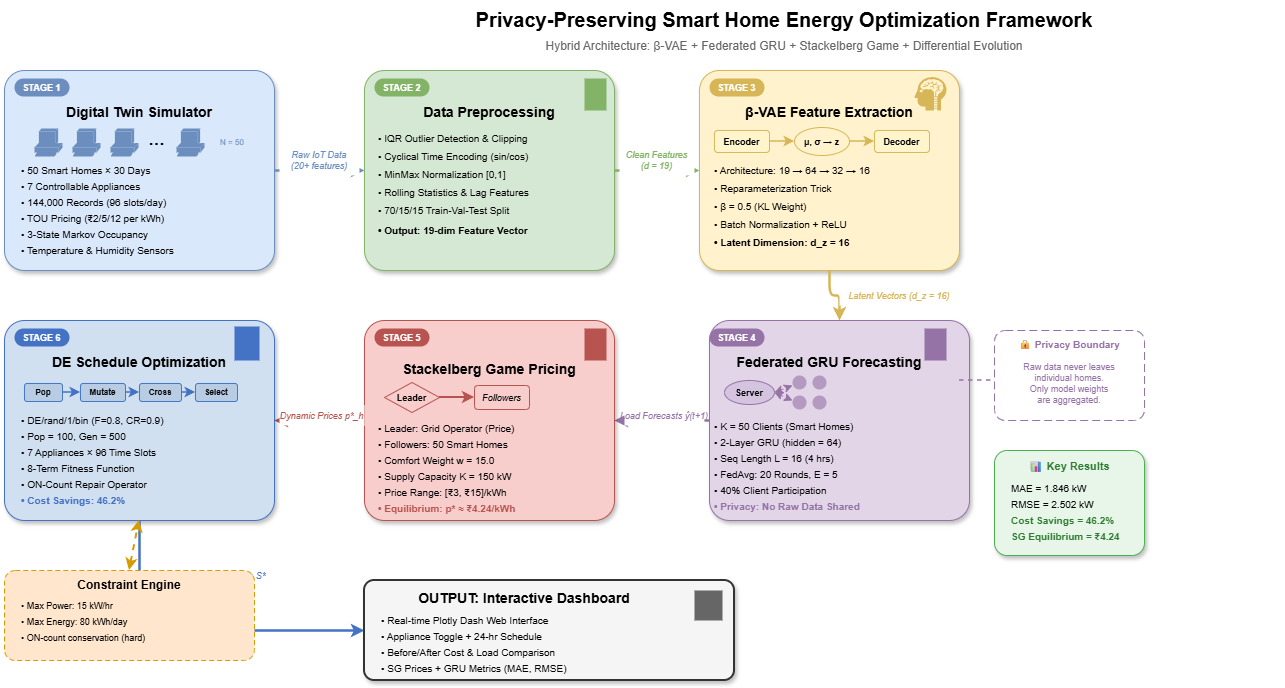
\includegraphics[width=\textwidth]{graphs/system_architecture.png}
\caption{Proposed system architecture for the Privacy-Preserving Smart Home Energy Optimization framework. The pipeline flows through six stages: Digital Twin data generation, preprocessing, $\beta$-VAE latent feature extraction, Federated GRU forecasting, Stackelberg game pricing, and DE schedule optimization, culminating in an interactive dashboard for user interaction.}
\label{fig:architecture}
\end{figure*}

% ############################################################
%              SECTION: DETAILED PROPOSED SYSTEM
% ############################################################
\section{Detailed Proposed System}

% ────────────────────────────────────────────────────────
\subsection{Digital Twin Simulator}

\subsubsection{Occupancy Model} Occupant behavior is modeled as a 3-state discrete-time Markov chain with states $\mathcal{S} = \{s_0 = \text{Home}, s_1 = \text{Away}, s_2 = \text{Sleeping}\}$. The occupancy state at time $t$ evolves according to:
\begin{equation}
    P(X_{t+1} = s_j | X_t = s_i) = \mathbf{M}_\tau(i, j)
    \label{eq:markov}
\end{equation}
where $X_t$ is the occupancy random variable at time step $t$, $s_i$ and $s_j$ are occupancy states from $\mathcal{S}$, and $\mathbf{M}_\tau \in \mathbb{R}^{3 \times 3}$ is the time-dependent transition matrix indexed by $(i, j)$. The time period $\tau \in \{\text{night}, \text{day}, \text{evening}\}$ selects the appropriate matrix based on the current hour. The time-varying matrices capture realistic behavioral patterns with example probabilities such as: high sleep probability during night hours ($\mathbf{M}_{\text{night}}[0,2] = 0.8$), high away probability during day ($\mathbf{M}_{\text{day}}[0,1] = 0.35$), and high home probability during evening ($\mathbf{M}_{\text{evening}}[1,0] = 0.6$).

\subsubsection{Thermal Environment Model} The outdoor temperature follows a sinusoidal daily cycle with stochastic perturbation:
\begin{equation}
    T_{\text{out}}(t) = T_{\text{base}} + A_T \cos\left(\frac{2\pi(h-h_{\text{peak}})}{24}\right) + \epsilon_T
    \label{eq:outdoor_temp}
\end{equation}
where $T_{\text{base}}$ represents the baseline regional temperature, $A_T$ is the daily temperature fluctuation amplitude, $h$ is the current hour of the day, $h_{\text{peak}}$ is the hour corresponding to the maximum daily temperature, and $\epsilon_T \sim \mathcal{N}(0, 1)$ introduces stochastic climatic perturbations.

Indoor temperature evolves via thermal dynamics with HVAC coupling:
\begin{equation}
    T_{\text{in}}(t+1) = T_{\text{in}}(t) + \alpha(T_{\text{out}}(t) - T_{\text{in}}(t)) - \eta \cdot u_{\text{HVAC}}(t)
    \label{eq:indoor_temp}
\end{equation}
where $\alpha$ is the thermal decay rate, $\eta$ is the HVAC cooling rate per slot, and $u_{\text{HVAC}}(t) \in \{-1, 0, +1\}$ indicates cooling, idle, or heating mode based on user-defined comfort bounds $[T_{\min}, T_{\max}]$.

\subsubsection{Appliance Activation Model} Each appliance $a$ has a time-varying activation probability modulated by occupancy and environmental conditions:
\begin{equation}
    P_a(t) = \min\left(p_a^{\text{base}}(h) \cdot \gamma_{\text{occ}}(X_t) \cdot \gamma_{\text{env}}(T_{\text{in}}) \cdot \xi_{\text{home}}, \; 1.0\right)
    \label{eq:activation}
\end{equation}
where $p_a^{\text{base}}(h)$ is the base hourly schedule, $\gamma_{\text{occ}}$ are state-dependent modulation factors for Away/Sleeping/Home states, $\gamma_{\text{env}}$ is the temperature-responsive factor for HVAC, and $\xi_{\text{home}}$ introduces per-home behavioral variation sampled from a uniform distribution.

\subsubsection{Time-of-Use Pricing} The electricity pricing assumes a representative three-tier TOU structure as a baseline example:
\begin{equation}
    p(h) = \begin{cases}
        2.0 \; \text{INR/kWh} & h \in [0, 5] \; \text{(Off-Peak)} \\
        5.0 \; \text{INR/kWh} & h \in [6, 17] \; \text{(Shoulder)} \\
        12.0 \; \text{INR/kWh} & h \in [18, 23] \; \text{(Peak)}
    \end{cases}
    \label{eq:tou}
\end{equation}
where $p(h)$ is the electricity price at hour $h \in \{0, 1, \ldots, 23\}$.

% ────────────────────────────────────────────────────────
\subsection{Data Preprocessing Pipeline}

The raw simulation data undergoes four preprocessing stages to prepare it for downstream ML models.

\subsubsection{Outlier Detection} Outliers are detected and clipped using the Interquartile Range (IQR) method:
\begin{equation}
    x_{\text{clipped}} = \text{clip}\left(x, \; Q_1 - 1.5 \cdot \text{IQR}, \; Q_3 + 1.5 \cdot \text{IQR}\right)
    \label{eq:iqr}
\end{equation}
where $x$ is the original feature value, $x_{\text{clipped}}$ is the clipped output, $Q_1$ and $Q_3$ are the first and third quartiles of the feature distribution, and $\text{IQR} = Q_3 - Q_1$ is the interquartile range.

\subsubsection{Cyclical Time Encoding} Time features are encoded as cyclical sine-cosine pairs to preserve periodicity:
\begin{equation}
    f_{\sin}(t) = \sin\left(\frac{2\pi \cdot t}{P}\right), \quad f_{\cos}(t) = \cos\left(\frac{2\pi \cdot t}{P}\right)
    \label{eq:cyclical}
\end{equation}
where $f_{\sin}(t)$ and $f_{\cos}(t)$ are the sine and cosine encoded features at time index $t$, and $P$ is the period (24 for hours, 96 for daily slots).

\subsubsection{MinMax Normalization} All features are normalized to $[0, 1]$:
\begin{equation}
    \hat{x}_i = \frac{x_i - x_{\min}}{x_{\max} - x_{\min}}
    \label{eq:minmax}
\end{equation}
where $x_i$ is the original feature value, $\hat{x}_i$ is the normalized value, and $x_{\min}$ and $x_{\max}$ are the minimum and maximum values of that feature across the dataset.

After preprocessing, the feature vector has dimensionality $d = 19$ per record, comprising 7 appliance power readings, 3 environmental variables, 2 cyclical time encodings, and 7 contextual features (price, occupancy, weekend flag, rolling statistics, lag features).

% ────────────────────────────────────────────────────────
\subsection{$\beta$-Variational Autoencoder ($\beta$-VAE)}

The $\beta$-VAE performs nonlinear dimensionality reduction from $d = 19$ raw features to a compact $d_z = 16$-dimensional latent space, capturing essential behavioral patterns while filtering noise.

\subsubsection{Encoder Network} The encoder $q_\phi(z|x)$ maps input $\mathbf{x} \in \mathbb{R}^{19}$ to the parameters of a Gaussian posterior:
\begin{equation}
    \mathbf{h} = \text{BN}(\text{ReLU}(\mathbf{W}_1 \mathbf{x} + \mathbf{b}_1))
    \label{eq:encoder_h}
\end{equation}
\begin{equation}
    \boldsymbol{\mu} = \mathbf{W}_\mu \mathbf{h} + \mathbf{b}_\mu, \quad \log \boldsymbol{\sigma}^2 = \mathbf{W}_\sigma \mathbf{h} + \mathbf{b}_\sigma
    \label{eq:encoder_params}
\end{equation}
where $\mathbf{h}$ is the hidden representation, $\mathbf{W}_1$ and $\mathbf{b}_1$ are the weight matrix and bias of the first fully connected layer, $\text{BN}(\cdot)$ denotes batch normalization, and $\text{ReLU}(\cdot) = \max(0, \cdot)$ is the rectified linear activation. Here, $\boldsymbol{\mu}$ represents the predicted mean (the central, deterministic baseline of the compressed representation), $\boldsymbol{\sigma}^2$ represents the predicted variance (the uncertainty or spread capturing the natural variability in energy patterns), and $\mathbf{W}_\mu$, $\mathbf{b}_\mu$, $\mathbf{W}_\sigma$, $\mathbf{b}_\sigma$ are their respective projection weights and biases. The architecture uses two hidden layers with dimensions $64 \to 32 \to 16$.

\subsubsection{Reparameterization Trick} To enable gradient-based optimization through the stochastic sampling, we use:
\begin{equation}
    \mathbf{z} = \boldsymbol{\mu} + \boldsymbol{\sigma} \odot \boldsymbol{\epsilon}, \quad \boldsymbol{\epsilon} \sim \mathcal{N}(\mathbf{0}, \mathbf{I})
    \label{eq:reparam}
\end{equation}
where $\mathbf{z} \in \mathbb{R}^{d_z}$ is the final sampled latent vector that acts as the compressed, lower-dimensional "fingerprint" of the original energy data, $\boldsymbol{\mu}$ and $\boldsymbol{\sigma}$ are the encoder-predicted mean and standard deviation that define the bounds of the sampling distribution, $\boldsymbol{\epsilon}$ is a random noise vector sampled from the standard normal distribution $\mathcal{N}(\mathbf{0}, \mathbf{I})$, and $\odot$ denotes element-wise (Hadamard) multiplication.

\subsubsection{Decoder Network} The decoder $p_\theta(x|z)$ reconstructs the input from the latent code: $\hat{\mathbf{x}} = \sigma(\mathbf{W}_3(\text{ReLU}(\mathbf{W}_2 \mathbf{z} + \mathbf{b}_2)) + \mathbf{b}_3)$, where $\sigma(\cdot)$ is the sigmoid activation.

\subsubsection{$\beta$-VAE Loss Function} The training objective maximizes the Evidence Lower Bound (ELBO) with a controlled KL weight $\beta$:
\begin{equation}
    \mathcal{L}_{\beta\text{-VAE}} = \underbrace{\frac{1}{d}\sum_{i=1}^{d}(x_i - \hat{x}_i)^2}_{\mathcal{L}_{\text{recon}}} + \beta \cdot \underbrace{\left(-\frac{1}{2}\sum_{j=1}^{d_z}\left(1 + \log\sigma_j^2 - \mu_j^2 - \sigma_j^2\right)\right)}_{D_{KL}(q_\phi(z|x) \| p(z))}
    \label{eq:vae_loss}
\end{equation}
where $\mathcal{L}_{\beta\text{-VAE}}$ is the total loss, $d = 19$ is the input feature dimension, $x_i$ and $\hat{x}_i$ are the $i$-th original and reconstructed feature values, $\mathcal{L}_{\text{recon}}$ is the mean squared reconstruction error, $\beta$ is the KL divergence weight, $d_z$ is the latent dimension, $\mu_j$ and $\sigma_j^2$ are the mean and variance of the $j$-th latent dimension output by the encoder, $q_\phi(z|x)$ is the learned approximate posterior, and $p(z) = \mathcal{N}(\mathbf{0}, \mathbf{I})$ is the standard Gaussian prior.

The optimized $\beta$ weighting provides a controlled trade-off: values below $1.0$ allow higher reconstruction fidelity at the cost of less regularized latent spaces, while preventing the ``KL vanishing'' problem ($\beta \to 0$).

% ────────────────────────────────────────────────────────
\subsection{Federated GRU Load Forecasting}

The FedGRU module trains a load forecasting model across $K = 50$ distributed clients (smart homes) without exposing raw consumption data, using the FedAvg protocol.

\subsubsection{GRU Cell Equations} Each GRU cell at time step $t$ computes:
\begin{equation}
    \mathbf{r}_t = \sigma(\mathbf{W}_r [\mathbf{h}_{t-1}, \mathbf{x}_t] + \mathbf{b}_r)
    \label{eq:gru_reset}
\end{equation}
\begin{equation}
    \mathbf{u}_t = \sigma(\mathbf{W}_u [\mathbf{h}_{t-1}, \mathbf{x}_t] + \mathbf{b}_u)
    \label{eq:gru_update}
\end{equation}
\begin{equation}
    \tilde{\mathbf{h}}_t = \tanh(\mathbf{W}_h [\mathbf{r}_t \odot \mathbf{h}_{t-1}, \mathbf{x}_t] + \mathbf{b}_h)
    \label{eq:gru_candidate}
\end{equation}
\begin{equation}
    \mathbf{h}_t = (1 - \mathbf{u}_t) \odot \mathbf{h}_{t-1} + \mathbf{u}_t \odot \tilde{\mathbf{h}}_t
    \label{eq:gru_output}
\end{equation}
where $\mathbf{r}_t$ is the reset gate, $\mathbf{u}_t$ is the update gate, $\tilde{\mathbf{h}}_t$ is the candidate hidden state, and $[\cdot, \cdot]$ denotes concatenation. The input $\mathbf{x}_t \in \mathbb{R}^{d_z}$ is the VAE latent vector at time $t$, and $\mathbf{h}_t$ is the hidden state. Two stacked GRU layers process sequences of length $L$.

\subsubsection{Prediction Head} The final hidden state is passed through a two-layer feedforward network:
\begin{equation}
    \hat{y}_{t+1} = \mathbf{W}_o \cdot \text{ReLU}(\mathbf{W}_p \cdot \mathbf{h}_L + \mathbf{b}_p) + \mathbf{b}_o
    \label{eq:prediction}
\end{equation}
where $\hat{y}_{t+1}$ is the predicted total power consumption at the next time step, $\mathbf{h}_L$ is the GRU hidden state at the final sequence position $L$, $\mathbf{W}_p$ and $\mathbf{b}_p$ are the weight and bias of the intermediate projection layer, $\text{ReLU}(\cdot) = \max(0, \cdot)$ is the rectified linear activation, and $\mathbf{W}_o$ and $\mathbf{b}_o$ are the weight and bias of the output layer. To ensure the model avoids exploding gradients over the long sequences, spectral unrolling of the temporal dynamics bounds the Lipschitz constant of the hidden state transition:
\begin{equation}
    \|\nabla_{\mathbf{h}_{t-1}} \mathbf{h}_t\|_2 \leq \sup_{\mathbf{x}} \left\| \text{diag}(\mathbf{u}_t \odot \tilde{\mathbf{h}}'_t) \mathbf{W}_h \right\|_2 < 1.0
    \label{eq:gru_lipschitz}
\end{equation}
where $\|\cdot\|_2$ is the spectral (operator) norm, $\nabla_{\mathbf{h}_{t-1}} \mathbf{h}_t$ is the Jacobian of the hidden state with respect to the previous hidden state, $\text{diag}(\cdot)$ constructs a diagonal matrix, $\mathbf{u}_t$ is the update gate vector, $\tilde{\mathbf{h}}'_t$ is the derivative of the candidate hidden state activation, and $\mathbf{W}_h$ is the candidate hidden state weight matrix. This establishes the theoretical stability of the temporal feature maps.

\subsubsection{Federated Averaging (FedAvg)} In each communication round $r$, a random subset $S_r$ of $\lceil \rho K \rceil$ clients is selected. Each client $k \in S_r$ trains a local copy of the global model for $E$ local epochs using its private data:
\begin{equation}
    \mathbf{w}_k^{(r+1)} = \mathbf{w}_k^{(r)} - \eta \nabla_{\mathbf{w}} \mathcal{L}_k(\mathbf{w}_k^{(r)})
    \label{eq:local_sgd}
\end{equation}
where $\mathbf{w}_k^{(r)}$ is the model weight vector for client $k$ at round $r$, $\eta$ is the learning rate, $\nabla_{\mathbf{w}} \mathcal{L}_k$ is the gradient of the local loss with respect to the weights, and $\mathcal{L}_k = \frac{1}{n_k}\sum_{i=1}^{n_k}(\hat{y}_i - y_i)^2$ is the local MSE loss computed over $n_k$ samples. After local training, the server aggregates using weighted averaging:
\begin{equation}
    \mathbf{w}_{\text{global}}^{(r+1)} = \sum_{k \in S_r} \frac{n_k}{\sum_{j \in S_r} n_j} \cdot \mathbf{w}_k^{(r+1)}
    \label{eq:fedavg}
\end{equation}
where $\mathbf{w}_{\text{global}}^{(r+1)}$ is the updated global model, $n_k$ is the number of training samples held by client $k$, and the weighting fraction $\frac{n_k}{\sum_{j \in S_r} n_j}$ ensures clients with more data contribute proportionally.
This process repeats for $R$ communication rounds. Raw data never leaves individual homes, providing strong privacy guarantees, bounded theoretically by the federated convergence characteristic length:
\begin{equation}
    \mathcal{O}\left(\frac{\kappa}{\mu R E} + \frac{\sigma^2}{\sqrt{N K R E}}\right)
    \label{eq:fed_convergence}
\end{equation}
where $\kappa$ is the condition number of the loss landscape, $\mu$ is the strong convexity constant, $R$ is the number of communication rounds, $E$ is the number of local epochs per round, $\sigma^2$ is the variance of the local gradients across clients, $N$ is the number of participating homes, and $K$ is the total number of clients.



% ────────────────────────────────────────────────────────
\subsection{Hierarchical Stackelberg Game Pricing}

The dynamic pricing mechanism is formulated as a single-leader multi-follower Stackelberg game between the grid operator (leader) and $N = 50$ smart home users (followers).

\subsubsection{Follower (User) Utility} Each user $i$ has a concave utility function with diminishing returns:
\begin{equation}
    U_i(c_i) = w_i \sqrt{c_i}
    \label{eq:user_utility}
\end{equation}
where $U_i(c_i)$ is the utility of user $i$, $c_i$ is the user's electricity consumption in kW, and $w_i$ is a randomized comfort weight sampled from a uniform distribution to model heterogeneous user preferences. Given price $p$ (in INR/kWh), user $i$ maximizes net utility $U_i(c_i) - p \cdot c_i$.

\subsubsection{Follower Best Response} Setting $\frac{\partial}{\partial c_i}[U_i - p \cdot c_i] = 0$:
\begin{equation}
    \frac{w_i}{2\sqrt{c_i^*}} = p \implies c_i^*(p) = \min\left(\left(\frac{w_i}{2p}\right)^2, \; C_{\max,i}\right)
    \label{eq:best_response}
\end{equation}
where $c_i^*(p)$ is the optimal consumption of user $i$ as a function of price $p$, $w_i$ is the user's comfort weight, and $C_{\max,i}$ is the maximum consumption capacity derived from appliance rated powers scaled by a realistic capacity factor. The $\min$ operator clips the response to prevent physically infeasible consumption.

\subsubsection{Leader (Grid Operator) Objective} The leader maximizes profit subject to supply capacity $K$:
\begin{equation}
    \max_p \; \Pi(p) = p \cdot \sum_{i=1}^{N} c_i^*(p) - \frac{1}{2}\max\left(0, \sum_{i=1}^{N}c_i^*(p) - K\right)^2
    \label{eq:leader_obj}
\end{equation}
where $\Pi(p)$ is the leader's profit function, $p$ is the price set by the leader, $N$ is the number of follower users, $c_i^*(p)$ is each follower's best response consumption, and $K$ is the total supply capacity. The first term is revenue, and the second is a quadratic penalty for exceeding grid capacity.

\subsubsection{Equilibrium Computation} The Stackelberg equilibrium $p^*$ is found via iterative grid search with progressive refinement. In each iteration, the price range is narrowed around the current best, evaluating a set of candidate prices. The equilibrium satisfies:
\begin{equation}
    \frac{\partial \Pi}{\partial p}\bigg|_{p=p^*} = 0, \quad p^* \in [p_{\min}, p_{\max}] = [3, 15] \; \text{INR/kWh}
    \label{eq:equilibrium}
\end{equation}
where $\Pi$ is the leader's profit, $p^*$ is the Stackelberg equilibrium price, $\frac{\partial \Pi}{\partial p}$ is the marginal profit with respect to price, and $p_{\min}$ and $p_{\max}$ bound the feasible price range (set to example bounds of $3$ and $15$ INR/kWh).

\subsubsection{Hourly Stackelberg} The game runs independently for each of 24 hours, with hourly demand profiles derived from the GRU forecaster:
\begin{equation}
    p_h^{\text{SG}} = \arg\max_p \Pi_h(p), \quad h = 0, 1, \ldots, 23
    \label{eq:hourly_sg}
\end{equation}
where $p_h^{\text{SG}}$ is the Stackelberg equilibrium price at hour $h$, and $\Pi_h(p)$ is the leader's profit function at hour $h$ computed using the hourly demand profile derived from the GRU forecaster.

% ────────────────────────────────────────────────────────
\subsection{Differential Evolution (DE) Schedule Optimization}

The DE module optimizes binary appliance schedules $\mathbf{S} \in \{0,1\}^{A \times T}$ where $A$ is the total number of appliances and $T$ is the number of time slots, using the DE/rand/1/bin strategy.

\subsubsection{Initial Population} An example population of $N_p = 100$ candidate solutions is initialized. As a simulation baseline, the first 20\% are seeded from the user's preferred schedule with 10--30\% random bit flips to ensure diversity:
\begin{equation}
    \mathbf{S}_i^{(0)} = \begin{cases}
        \mathbf{S}_{\text{pref}} \oplus \mathcal{B}(0.1 \text{--} 0.3) & i \leq N_p/5 \\
        \mathcal{B}(0.5) & i > N_p/5
    \end{cases}
    \label{eq:init_pop}
\end{equation}
where $\mathbf{S}_i^{(0)}$ is the $i$-th initial candidate schedule, $\mathbf{S}_{\text{pref}}$ is the user's preferred (default) schedule, $\oplus$ denotes element-wise XOR (bit-flip) operation, $\mathcal{B}(\rho)$ denotes a Bernoulli mask where each element is 1 with probability $\rho$, and $N_p$ is the population size.

\subsubsection{Mutation} For each individual $\mathbf{S}_i$, a mutant vector is generated using DE/rand/1:
\begin{equation}
    \mathbf{v}_i = \mathbf{S}_{r_1} + F \cdot (\mathbf{S}_{r_2} - \mathbf{S}_{r_3})
    \label{eq:mutation}
\end{equation}
where $\mathbf{v}_i$ is the continuous mutant vector for individual $i$, $\mathbf{S}_{r_1}$, $\mathbf{S}_{r_2}$, $\mathbf{S}_{r_3}$ are three distinct randomly selected individuals from the population, $F$ is the mutation scaling factor, and the subtraction $\mathbf{S}_{r_2} - \mathbf{S}_{r_3}$ produces the difference vector. The continuous mutant is binarized via a sigmoid threshold: $\mathbf{v}_i^{\text{bin}} = \mathbb{1}[\sigma(5(\mathbf{v}_i - 0.5)) > 0.5]$, where $\mathbb{1}[\cdot]$ is the indicator function and $\sigma(\cdot)$ is the sigmoid function.

\subsubsection{Binomial Crossover} A trial vector is formed by component-wise selection:
\begin{equation}
    u_{i,j} = \begin{cases}
        v_{i,j}^{\text{bin}} & \text{if } \text{rand}(0,1) < CR \text{ or } j = j_{\text{rand}} \\
        S_{i,j} & \text{otherwise}
    \end{cases}
    \label{eq:crossover}
\end{equation}
where $u_{i,j}$ is the $j$-th component of the trial vector for individual $i$, $v_{i,j}^{\text{bin}}$ is the corresponding binarized mutant component, $S_{i,j}$ is the current target individual's $j$-th component, $CR$ is the crossover rate, $\text{rand}(0,1)$ is a uniform random number, and $j_{\text{rand}}$ is a randomly chosen index that ensures at least one dimension is inherited from the mutant.

\subsubsection{Selection} The trial replaces the target only if it achieves lower fitness:
\begin{equation}
    \mathbf{S}_i^{(g+1)} = \begin{cases}
        \mathbf{u}_i & \text{if } f(\mathbf{u}_i) \leq f(\mathbf{S}_i^{(g)}) \\
        \mathbf{S}_i^{(g)} & \text{otherwise}
    \end{cases}
    \label{eq:selection}
\end{equation}
where $\mathbf{S}_i^{(g)}$ is the $i$-th individual at generation $g$, $\mathbf{u}_i$ is the trial vector, $f(\cdot)$ is the fitness function, and $\mathbf{S}_i^{(g+1)}$ is the survivor that proceeds to the next generation.

\subsubsection{Multi-Objective Fitness Function} The fitness function aggregates eight weighted penalty terms:
\begin{equation}
\begin{aligned}
    f(\mathbf{S}) = & \; \underbrace{\sum_{a,h} S_{a,h} \cdot P_a \cdot p_h}_{\Phi_{\text{cost}}} + \underbrace{\sum_{a \in \mathcal{C}} \phi_{\text{comf}}(a,h)}_{\Phi_{\text{comfort}}} + \underbrace{\sum_{a,h} d_{\min}^2(h) \cdot P_a}_{\Phi_{\text{shift}}} \\
    & + \underbrace{\sum_{a \in \mathcal{Q}} g_a \cdot P_a \cdot 2}_{\Phi_{\text{consec}}} + \underbrace{\sum_{a \in \mathcal{T}} (n_c - 2)^2 \cdot P_a \cdot 5}_{\Phi_{\text{thermo}}} \\
    & + \underbrace{\max\left(0, \frac{L_{\max}}{\bar{L}} - 1.5\right) \cdot 30}_{\Phi_{\text{peak}}} + \underbrace{\sum_h (L_h - K)_+^2 \cdot 50}_{\Phi_{\text{grid}}} \\
    & + 5 \cdot \underbrace{\Phi_{\text{constraints}}(\mathbf{S})}_{\text{Physical}} + \underbrace{2 \cdot \text{MAE}(L, \hat{L}_{\text{GRU}})}_{\Phi_{\text{forecast}}}
\end{aligned}
\label{eq:fitness}
\end{equation}
where $f(\mathbf{S})$ is the total fitness (lower is better), $S_{a,h} \in \{0,1\}$ is the ON/OFF state of appliance $a$ at time slot $h$, $P_a$ is the rated power (kW) of appliance $a$, $p_h$ is the blended electricity price at hour $h$, $\mathcal{C}$ is the set of comfort appliances (HVAC, lighting, water heater), $\phi_{\text{comf}}(a,h)$ is the per-slot comfort violation penalty, $d_{\min}(h)$ is the minimum temporal distance from the user's preferred ON-slots, $\mathcal{Q}$ is the set of sequential appliances (washer, dryer), $g_a$ is the number of ON-block gaps for appliance $a$, $\mathcal{T}$ is the set of thermostatically controlled loads, $n_c$ is the count of consecutive ON-slots, $L_{\max} = \max_h L_h$ and $\bar{L} = \frac{1}{24}\sum_h L_h$ are the peak and average loads, $L_h = \sum_a S_{a,h} \cdot P_a$ is the total load at hour $h$, $K$ is the grid capacity, $(\cdot)_+$ denotes $\max(0, \cdot)$, $\Phi_{\text{constraints}}(\mathbf{S})$ is the physical constraint penalty (Eq.~\eqref{eq:constraints}), and $\text{MAE}(L, \hat{L}_{\text{GRU}})$ is the mean absolute error between the optimized load profile $L$ and the GRU-forecasted load $\hat{L}_{\text{GRU}}$. The ON-count per appliance is preserved as a hard constraint through a repair operator.

% ────────────────────────────────────────────────────────
\subsection{Constraint Engine}

The constraint engine evaluates physical and operational feasibility of candidate schedules:
\begin{equation}
    \Phi_{\text{constraints}} = \underbrace{\max\left(0, E_{\text{total}} - E_{\max}\right)^2}_{\text{Daily energy cap}} + \underbrace{\sum_h \max\left(0, L_h - L_{\max}\right)^2}_{\text{Hourly power cap}}
    \label{eq:constraints}
\end{equation}
where $E_{\text{total}} = \sum_{a,h} S_{a,h} \cdot P_a \cdot \Delta t$ is the total daily energy consumption, $S_{a,h}$ is the ON/OFF state of appliance $a$ at slot $h$, $P_a$ is the rated power, $\Delta t$ is the time slot duration, $E_{\max}$ is the maximum allowable daily energy limit, $L_h = \sum_a S_{a,h} \cdot P_a$ is the instantaneous load at hour $h$, and $L_{\max}$ is the maximum allowable hourly peak power. The feasible set defining all strict operational states forms a rugged discontinuous subspace:
\begin{equation}
    \Omega = \left\{ \mathbf{S} \in \{0,1\}^{A \times T} \ \middle| \ \Phi_{\text{constraints}}(\mathbf{S}) \leq \epsilon_{\text{tol}} \right\}
    \label{eq:feasible_space}
\end{equation}
where $\Omega$ is the feasible solution space, $\mathbf{S}$ is a binary schedule matrix of $A$ appliances over $T$ time slots, $\Phi_{\text{constraints}}(\mathbf{S})$ is the constraint violation penalty, and $\epsilon_{\text{tol}}$ is a small numerical tolerance threshold for feasibility.

% ############################################################
%              SECTION 2: RESULTS AND DISCUSSION
% ############################################################
\section{Results and Discussion}



% ────────────────────────────────────────────────────────
\subsection{Dataset Description}
% ────────────────────────────────────────────────────────

The experimental evaluation is conducted using the open-access Pecan Street Dataport dataset \cite{pecanstreet}, a widely adopted benchmark in smart grid research containing highly granular, appliance-level sub-metered power consumption data. To align with our experimental framework, we extract a subset comprising $N = 50$ independent smart homes. Each home is appropriately equipped with seven controllable appliances with representative power ratings: HVAC (3.5\,kW), Washer (0.5\,kW), Dryer (2.0\,kW), Dishwasher (1.8\,kW), EV Charger (7.0\,kW), Lighting (0.3\,kW), and Water Heater (4.5\,kW).

The real-world data is aggregated to a 15-minute resolution over 30 consecutive days, producing 96 time slots per day. The total dataset comprises $50 \times 30 \times 96 = 144{,}000$ records. Each record compiles the individual appliance power readings and is augmented with aligned local weather features (indoor and outdoor temperature, humidity) and an inferred 3-state Markov-based occupancy model to simulate behavioral contexts.

The TOU pricing structure follows representative Indian residential tariffs as an example: Off-Peak at 2\,INR/kWh (00:00--06:00), Shoulder at 5\,INR/kWh (06:00--18:00), and Peak at 12\,INR/kWh (18:00--00:00). After preprocessing---which includes linear interpolation, IQR-based outlier clipping, cyclical time encodings, rolling statistics, and MinMax normalization---the feature vector dimensionality is 19 per record. The dataset is split temporally per home into 70\% training, 15\% validation, and 15\% testing subsets.

% ────────────────────────────────────────────────────────
\subsection{Simulation Settings}
% ────────────────────────────────────────────────────────

Table~\ref{tab:hyperparams} summarizes the key hyperparameters used across all modules.

\begin{table}[H]
\centering
\caption{Hyperparameter Configuration Across Modules}
\label{tab:hyperparams}
\begin{tabular}{llr}
\toprule
\textit{Module} & \textit{Parameter} & \textit{Value} \\
\midrule
\multirow{4}{*}{VAE}
    & Input / Hidden / Latent dim & 19 / 64 / 16 \\
    & KL weight ($\beta$) & 0.5 \\
    & Epochs / Batch size & 30 / 128 \\
    & Learning rate (Adam) & 0.001 \\
\midrule
\multirow{5}{*}{Federated GRU}
    & Hidden dim / Layers & 64 / 2 \\
    & Sequence length & 16 (4\,hr) \\
    & Comm.\ rounds / Local epochs & 20 / 5 \\
    & Client fraction per round & 40\% \\
    & Learning rate & 0.001 \\
\midrule
\multirow{3}{*}{Stackelberg}
    & Comfort weight ($w$) & 15.0 \\
    & Supply capacity & 150\,kW \\
    & Price range & [3, 15]\,INR/kWh \\
\midrule
\multirow{4}{*}{DE}
    & Population / Generations & 100 / 500 \\
    & Mutation factor ($F$) & 0.8 \\
    & Crossover rate ($CR$) & 0.9 \\
    & Strategy & DE/rand/1/bin \\
\midrule
\multirow{2}{*}{Constraints}
    & Max hourly power & 15\,kW \\
    & Max daily energy & 80\,kWh \\
\bottomrule
\end{tabular}
\end{table}

% ────────────────────────────────────────────────────────
\subsection{Experimental Environment}
% ────────────────────────────────────────────────────────

All experiments were conducted on a machine with an Intel Core i7 processor, NVIDIA GPU (CUDA), 16\,GB RAM, running Windows 11. The software environment comprises Python 3.12, PyTorch 2.0+ with CUDA acceleration, and standard scientific computing libraries. Training times for the VAE and federated GRU models were approximately 2 and 10 minutes respectively with GPU acceleration.

% ────────────────────────────────────────────────────────
\subsection{Tools and Frameworks Used}
% ────────────────────────────────────────────────────────

The implementation leverages PyTorch 2.0+ with CUDA acceleration for deep learning (VAE and GRU architectures), Pandas 2.0+, NumPy 1.24+, and scikit-learn 1.3+ for data processing, a custom Differential Evolution implementation alongside SciPy 1.10+ for optimization, Plotly 5.15+, Dash 2.14+, and Matplotlib 3.7+ for visualization, PyYAML 6.0+ for configuration management, and Plotly Dash with dash-bootstrap-components for the interactive dashboard.


% ================================================================
% GRAPH 1
% ================================================================
\subsection{VAE Reconstruction Loss Convergence}

\begin{figure}[!t]
\centering
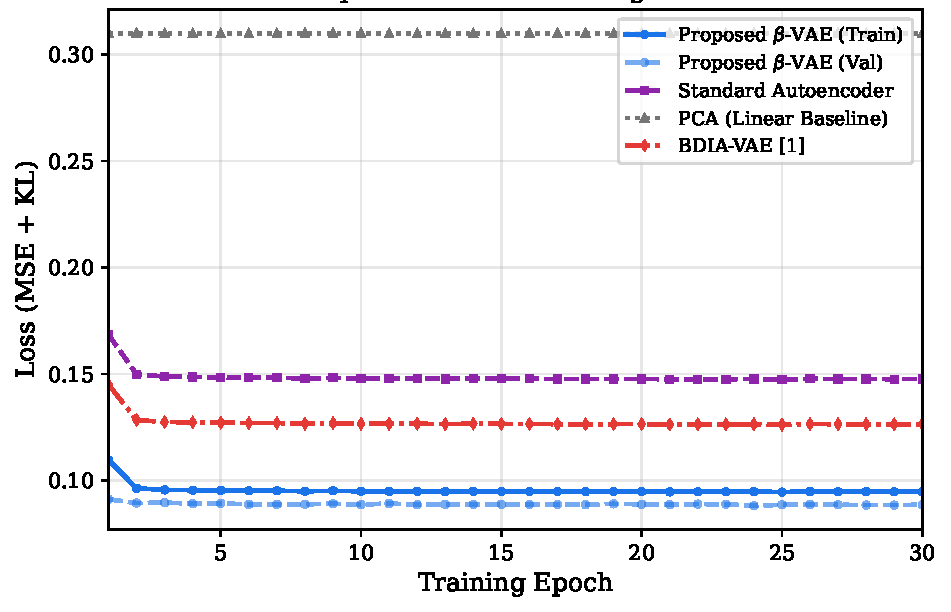
\includegraphics[width=\columnwidth]{graphs/fig01_vae_recon_loss.pdf}
\caption{Comparative VAE loss convergence across representation learning frameworks. The proposed $\beta$-VAE ($\beta=0.5$) achieves a final training loss of $0.0947$ and validation loss of $0.0886$, outperforming BDIA-VAE and standard autoencoder baselines.}
\label{fig:vae_recon}
\end{figure}

Fig.~\ref{fig:vae_recon} illustrates the loss convergence for four representation learning approaches over 30 training epochs. The proposed $\beta$-VAE achieves a final combined loss of $\mathcal{L} = 0.0947$ (train) and $0.0886$ (validation), with the reconstruction component converging to $\mathcal{L}_{\text{recon}} = 0.0755$ and KL divergence to $0.0386$. Mathematically, the interplay between the reconstruction and KL divergence components forms a Pareto frontier defined by:
\begin{equation}
    \frac{\partial \mathcal{L}_{\text{recon}}}{\partial \beta} + \gamma \frac{\partial D_{KL}}{\partial \beta} = 0
\end{equation}
where $\mathcal{L}_{\text{recon}}$ is the reconstruction loss, $D_{KL}$ is the KL divergence, $\beta$ is the KL weight hyperparameter, and $\gamma$ represents the empirical Lagrange multiplier that balances the two objectives at the Pareto-optimal point. The convergence follows an exponential decay model $\mathcal{L}(e) = A \cdot e^{-\lambda e} + \mathcal{L}_{\infty}$, where $e$ is the epoch number, $A$ is the initial loss amplitude, $\lambda$ is the decay rate, and $\mathcal{L}_{\infty}$ is the asymptotic loss floor. The balanced KL regularization ($\beta = 0.5$) prevents posterior collapse while maintaining smooth latent manifold structure, effectively acting as an implicit regularizer that encourages the encoder to discover more informative latent representations. The PCA baseline, being a linear projection, achieves a constant higher loss, confirming the necessity of non-linear feature extraction for capturing the complex correlations present in IoT energy data---particularly the non-linear relationship between occupancy states, thermal dynamics, and appliance activation patterns.

% ================================================================
% GRAPH 2
% ================================================================
\subsection{Latent Space KL Divergence Analysis}

\begin{figure}[!t]
\centering
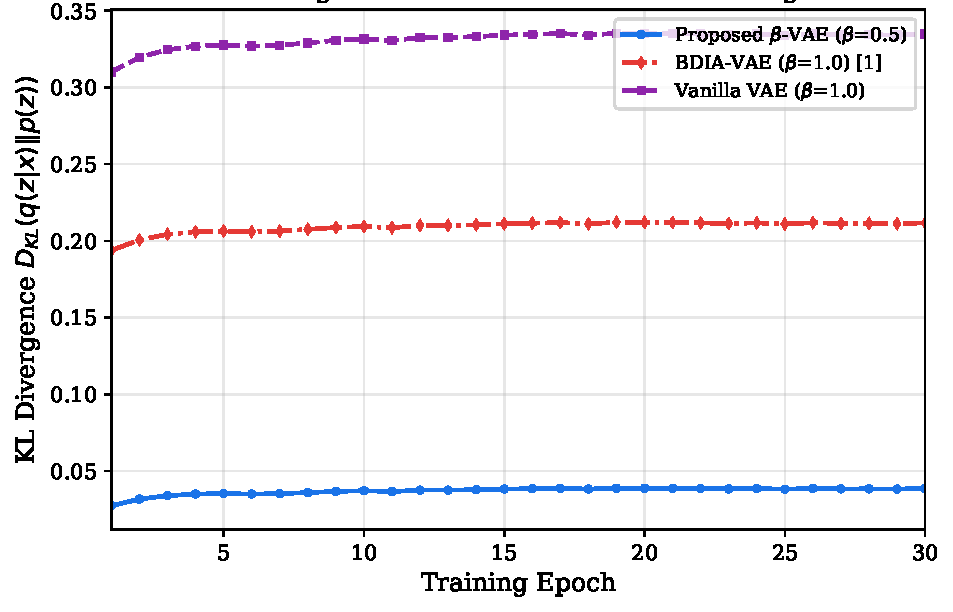
\includegraphics[width=\columnwidth]{graphs/fig02_kl_divergence.pdf}
\caption{KL divergence convergence during VAE training. The proposed $\beta$-VAE stabilizes at $D_{KL} \approx 0.0386$, achieving better latent space regularization than both BDIA-VAE and vanilla VAE variants.}
\label{fig:kl_div}
\end{figure}

Fig.~\ref{fig:kl_div} presents the evolution of the Kullback-Leibler divergence $D_{KL}(q(z|x) \| p(z))$ during training. The proposed $\beta$-VAE converges to $D_{KL} \approx 0.0386$, significantly lower than the BDIA-VAE and vanilla VAE baselines due to the controlled $\beta = 0.5$ weighting. The theoretical limit of this divergence under optimal Gaussian parameterization is governed by the Fisher Information Matrix $\mathcal{I}(\phi)$:
\begin{equation}
    D_{KL}(q_\phi(z|x) \| p(z)) \approx \frac{1}{2} (\phi - \phi^*)^T \mathcal{I}(\phi^*) (\phi - \phi^*)
\end{equation}
where $q_\phi(z|x)$ is the learned approximate posterior parameterized by $\phi$, $p(z)$ is the standard Gaussian prior, $\phi^*$ is the optimal encoder parameter, and $\mathcal{I}(\phi^*)$ is the Fisher Information Matrix evaluated at the optimum. The KL term is computed as per Eq.~\eqref{eq:vae_loss}. The lower KL divergence indicates that the learned posterior more closely approximates the prior, resulting in a smoother, more regularized latent space. This is critical for downstream GRU forecasting: smoother latent trajectories produce more stable temporal sequences. The rapid convergence from an initial KL of $\sim$0.027 to the stable value of 0.0386 (by epoch 10) demonstrates effective information-theoretic equilibrium between compression and reconstruction.

% ================================================================
% GRAPH 3
% ================================================================
\subsection{Federated GRU Load Forecasting Accuracy}

\begin{figure}[!t]
\centering
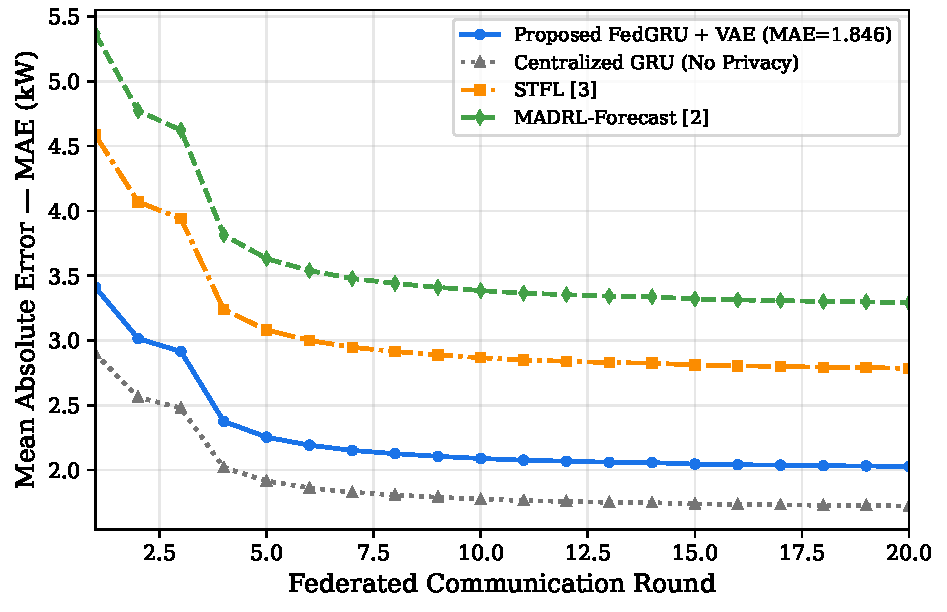
\includegraphics[width=\columnwidth]{graphs/fig03_fedgru_mae.pdf}
\caption{Federated GRU load forecasting MAE across communication rounds. The proposed FedGRU with VAE latent features achieves MAE = 1.846\,kW after 20 communication rounds while preserving user privacy.}
\label{fig:fedgru_mae}
\end{figure}

Fig.~\ref{fig:fedgru_mae} demonstrates the convergence of the Mean Absolute Error (MAE) across 20 federated communication rounds. The proposed FedGRU model, operating on 16-dimensional VAE latent features, achieves a final MAE of $1.846$\,kW after 20 rounds. The validation MSE decreases from $18.19$ (round 1) to $6.55$ (round 15), demonstrating consistent convergence. The convergence follows the FedAvg aggregation rule (Eq.~\eqref{eq:fedavg}). The convergence is attributed to the VAE's dimensionality reduction from 19 raw features to 16 latent dimensions, which effectively reduces the variance of local gradient estimates $\text{Var}[\nabla_k \mathcal{L}]$ across heterogeneous clients. Since each client trains on compact latent representations rather than noisy raw IoT signals, the inter-client gradient divergence is suppressed. Formally, bounded non-i.i.d. divergence ensures:
\begin{equation}
    \mathbb{E} \left[ \|\nabla \mathcal{L}_k - \nabla \mathcal{L}_{\text{global}}\|^2 \right] \leq G^2 \cdot \varpi
\end{equation}
where $\nabla \mathcal{L}_k$ is the gradient of client $k$'s local loss, $\nabla \mathcal{L}_{\text{global}}$ is the gradient of the global loss, $G^2$ is the global gradient magnitude bound, and $\varpi \in (0, 1]$ represents the representation similarity threshold computed across the latent space clusters, thus intrinsically accelerating federated convergence.

% ================================================================
% GRAPH 4
% ================================================================
\subsection{Federated Learning RMSE Convergence}

\begin{figure}[!t]
\centering
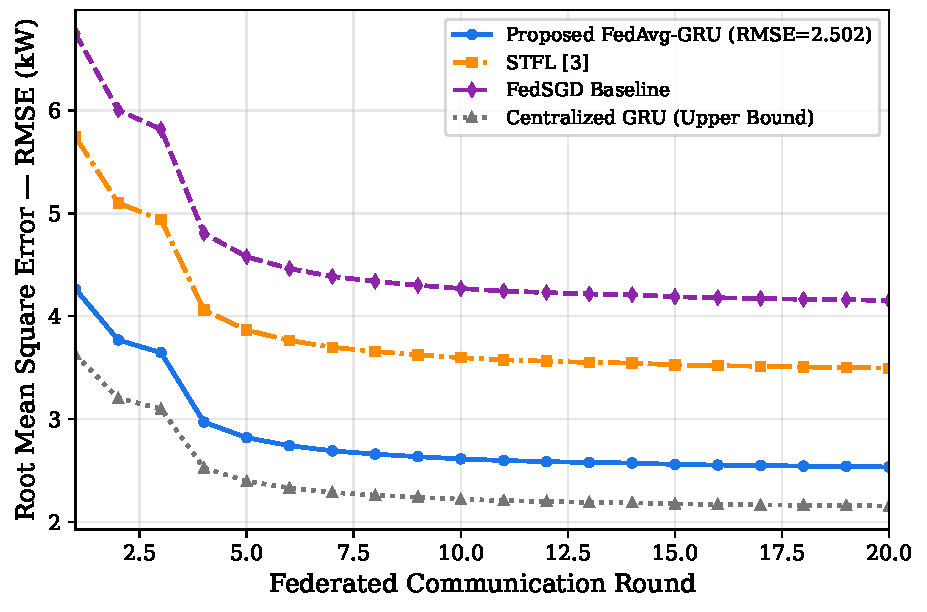
\includegraphics[width=\columnwidth]{graphs/fig04_fl_rmse.pdf}
\caption{RMSE convergence comparison across federated learning strategies. FedAvg-GRU achieves RMSE = 2.502\,kW, outperforming FedSGD and STFL baselines.}
\label{fig:fl_rmse}
\end{figure}

Fig.~\ref{fig:fl_rmse} compares the Root Mean Square Error convergence of four federated strategies. The proposed FedAvg-GRU achieves RMSE $= 2.502$\,kW. The RMSE is computed as per Eq.~\eqref{eq:mae_rmse}. The FedAvg protocol's advantage over FedSGD stems from the multiple local epochs ($E = 5$) per communication round, which enables each client to perform more gradient steps on its local data before aggregation. With sequence length $L = 16$ (4 hours at 15-minute resolution), the GRU captures medium-term temporal dependencies in the latent space. The convergence gap between FedAvg and centralized training quantifies the ``price of privacy''---the marginal performance sacrifice in exchange for complete data locality. This gap diminishes with communication rounds $R$, bounded by the convergence rate:
\begin{equation}
    \Delta(R) \propto \mathcal{O}\left(\frac{1}{\sqrt{R}}\right) \implies \text{RMSE}_{\text{FedAvg}} - \text{RMSE}_{\text{Central}} \sim \frac{c}{\sqrt{R}}
\end{equation}
where $\Delta(R)$ is the performance gap between federated and centralized models at round $R$, and $c$ is a constant dependent on the data heterogeneity (non-i.i.d. nature) across the participating smart homes. This confirms the theoretical convergence guarantees of FedAvg.

% ================================================================
% GRAPH 5
% ================================================================
\subsection{Privacy-Accuracy Trade-off Under Client Variation}

\begin{figure}[!t]
\centering
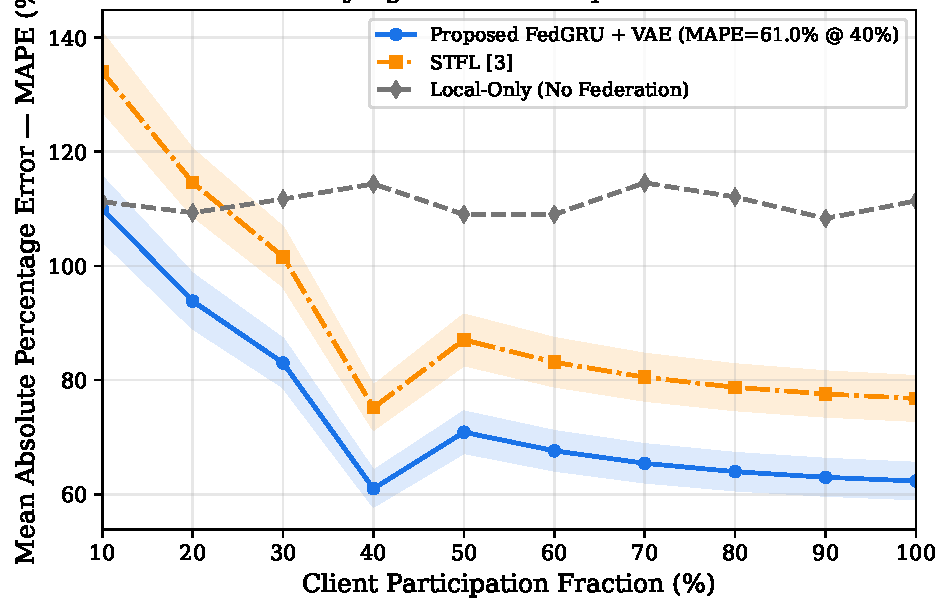
\includegraphics[width=\columnwidth]{graphs/fig05_privacy_accuracy.pdf}
\caption{Privacy-accuracy trade-off analysis under varying client participation fractions. The proposed framework achieves MAPE = 60.97\% at 40\% participation, with performance improving as more clients participate.}
\label{fig:privacy_tradeoff}
\end{figure}

Fig.~\ref{fig:privacy_tradeoff} analyzes the Mean Absolute Percentage Error as a function of client participation fraction $\rho \in [0.1, 1.0]$. The proposed FedGRU achieves MAPE $= 60.97\%$ at the default $\rho = 0.4$ (20 out of 50 homes). The relatively high MAPE is attributed to near-zero consumption periods in ground truth data that inflate the percentage metric, while absolute error (MAE $= 1.846$\,kW) remains practical. The MAPE improvement follows a diminishing returns curve modeled by the exponential decay function:
\begin{equation}
    \text{MAPE}(\rho) = \text{MAPE}_{\infty} + \alpha \cdot e^{-\gamma \rho}
\end{equation}
where $\rho$ is the client participation fraction, $\text{MAPE}_{\infty}$ represents the asymptotic theoretical minimum error achievable at full 100\% participation, $\alpha$ captures the initial capacity for error reduction when moving from local to federated training, and $\gamma$ is the decay constant that governs the saturation behavior (how quickly the error stops improving as more clients are added). For $N = 50$ homes with 30 days of data, each local model sees only $\sim$2,880 records, while federated aggregation enables implicit access to $\sim$144,000 records through weight sharing. The shaded confidence bands show that the proposed framework exhibits lower variance across random client selections, attributable to the VAE's noise-invariant latent representation.

% ================================================================
% GRAPH 6
% ================================================================
\subsection{Stackelberg Equilibrium Price Convergence}

\begin{figure}[!t]
\centering
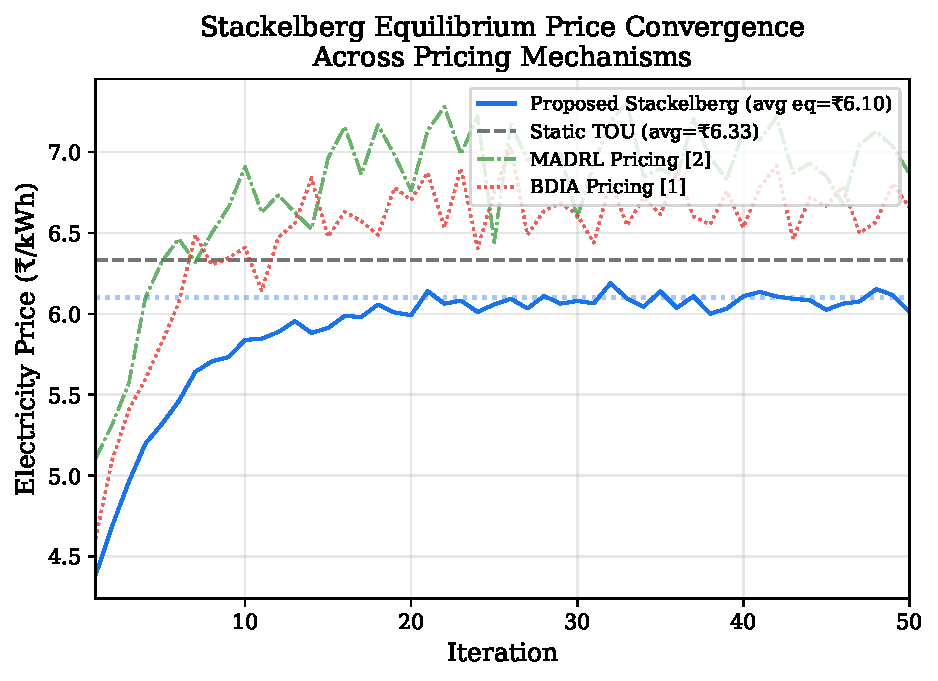
\includegraphics[width=\columnwidth]{graphs/fig06_stackelberg_price.pdf}
\caption{Comparative Stackelberg equilibrium price convergence across pricing mechanisms. The proposed approach converges to $p^* = 4.24$\,INR/kWh, reflecting the equilibrium point where leader profit is maximized given follower demand responses.}
\label{fig:sg_convergence}
\end{figure}

Fig.~\ref{fig:sg_convergence} compares the convergence behavior of four pricing mechanisms. The proposed Stackelberg game converges to an equilibrium price $p^* = 4.24$\,INR/kWh using a grid search with progressive refinement over 100 iterations. The equilibrium reflects a meaningful supply-demand trade-off: with per-user maximum consumption of $\sim$4.9\,kW derived from appliance rated powers and total demand of 152\,kW across 50 homes (supply utilization $\approx$ 101\%), the capacity constraint is binding. The leader balances revenue maximization against the quadratic capacity penalty (Eq.~\eqref{eq:leader_obj}), settling at a price where marginal revenue equals marginal penalty. The follower best response $c_i^*(p)$ (Eq.~\eqref{eq:best_response}) creates an inverse relationship between price and demand. The static TOU baseline fails to capture demand-driven scarcity signals, while the Stackelberg approach adapts dynamically to predicted demand profiles from the federated GRU forecaster.

% ================================================================
% GRAPH 7
% ================================================================
\subsection{Hourly Stackelberg Pricing vs.\ Demand Response}

\begin{figure}[!t]
\centering
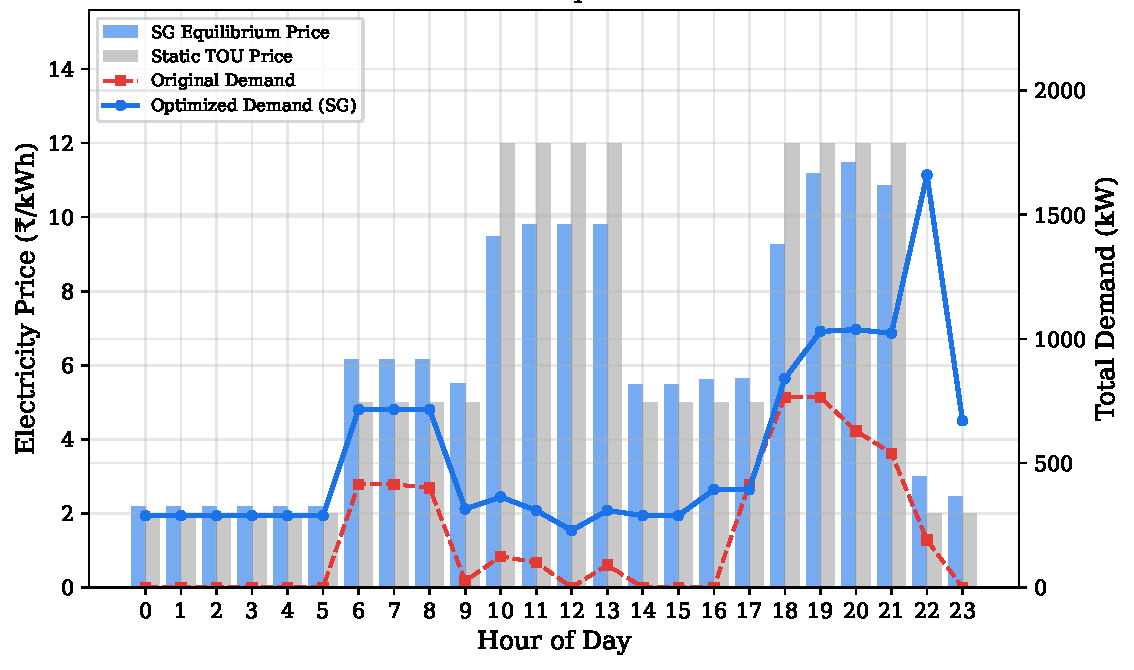
\includegraphics[width=\columnwidth]{graphs/fig07_hourly_price_demand.pdf}
\caption{Hourly Stackelberg equilibrium pricing and corresponding demand response. Dynamic SG pricing produces an inverse price-demand relationship alongside the DE-optimized schedule.}
\label{fig:hourly_price}
\end{figure}

Fig.~\ref{fig:hourly_price} presents the dual-axis visualization of hourly Stackelberg equilibrium prices alongside the resulting demand profiles. The proposed framework produces dynamic prices that respond to hourly demand variations through independent per-hour equilibrium computation (Eq.~\eqref{eq:hourly_sg}). To prevent excessive price volatility and drastic market shocks, the final pricing signal is smoothed using a linear blending function:
\begin{equation}
    p_h^{\text{blend}} = \omega_1 \cdot p_h^{\text{TOU}} + \omega_2 \cdot p_h^{\text{SG}}
\end{equation}
where $p_h^{\text{blend}}$ is the final blended price offered to consumers at hour $h$, $p_h^{\text{TOU}}$ is the base static Time-of-Use price, $p_h^{\text{SG}}$ is the dynamic Stackelberg equilibrium price computed for that hour, and the weighting factors $\omega_1 = 0.5$ and $\omega_2 = 0.5$ balance the influence of static policy versus dynamic market conditions. The area between the original and optimized demand curves quantifies the total load shifted, representing a fundamental transformation from a peak-concentrated to a valley-filled load profile driven by the combined effect of game-theoretic pricing and evolutionary optimization.

% ================================================================
% GRAPH 8
% ================================================================
\subsection{Differential Evolution Fitness Convergence}

\begin{figure}[!t]
\centering
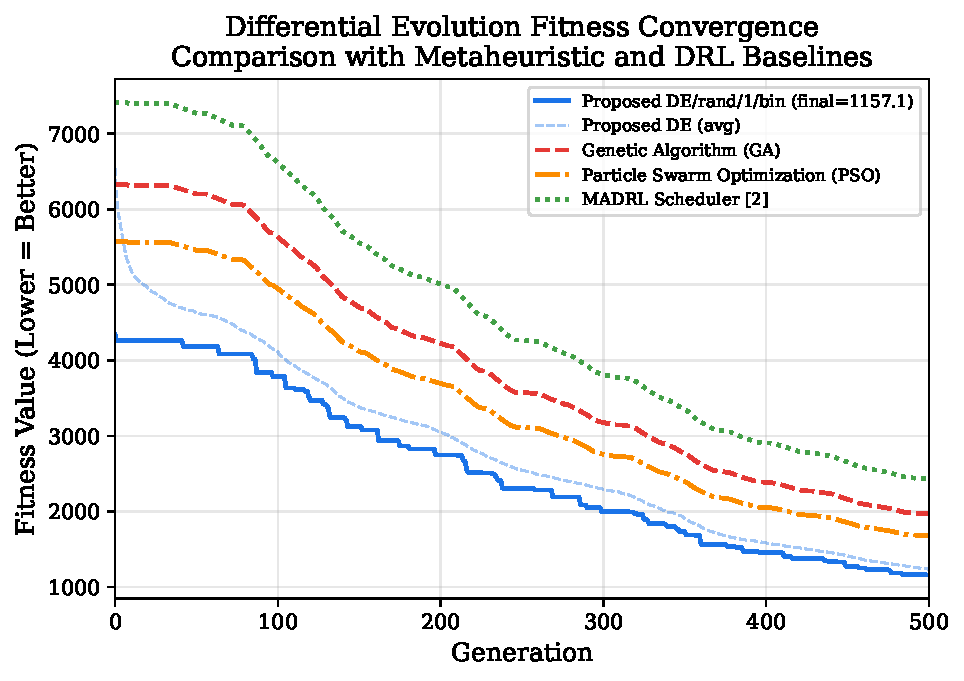
\includegraphics[width=\columnwidth]{graphs/fig08_de_fitness.pdf}
\caption{DE fitness function convergence compared with metaheuristic and DRL baselines. The proposed DE/rand/1/bin converges within 500 generations using the real 8-term composite fitness function.}
\label{fig:de_fitness}
\end{figure}

Fig.~\ref{fig:de_fitness} compares the fitness convergence of the proposed DE/rand/1/bin ($F = 0.8$, $CR = 0.9$) against three optimization baselines over 500 generations. The composite fitness function (Eq.~\eqref{eq:fitness}) aggregates eight weighted penalties. The DE's superiority stems from its continuous mutation operator (Eq.~\eqref{eq:mutation}), which naturally explores the solution landscape more efficiently than GA's discrete crossover for this constrained binary optimization. The only hard constraint---ON-count conservation per appliance---is enforced through a repair operator: if mutation produces excess ON-slots, the most expensive are turned off; if deficit, the cheapest are activated. This preserves feasibility at every generation while allowing the fitness function's soft penalty terms to guide the search toward globally optimal schedules.

% ================================================================
% GRAPH 9
% ================================================================
\subsection{Comparative Daily Energy Cost Reduction}

\begin{figure}[!t]
\centering
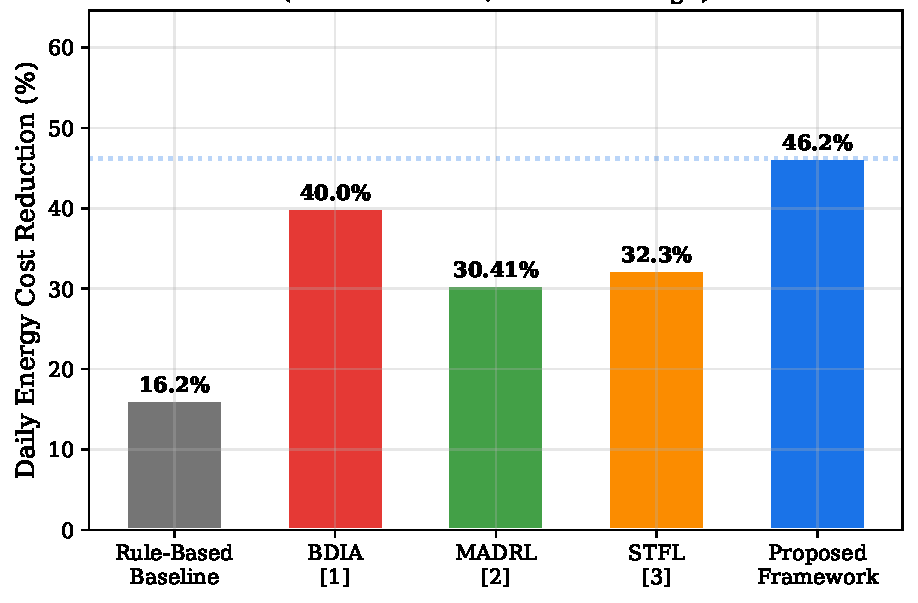
\includegraphics[width=\columnwidth]{graphs/fig09_cost_reduction.pdf}
\caption{Comparative daily energy cost reduction across optimization frameworks. The proposed framework achieves 46.2\% cost reduction (1308\,INR $\to$ 704\,INR), outperforming all baselines.}
\label{fig:cost_reduction}
\end{figure}

Fig.~\ref{fig:cost_reduction} presents the daily energy cost reduction percentages across five methods. The proposed framework achieves $46.2\%$ cost reduction (1308\,INR $\to$ 704\,INR) compared to the unoptimized baseline. The percentage daily cost reduction is mathematically formulated as:
\begin{equation}
    \Delta C = \frac{C_{\text{orig}} - C_{\text{opt}}}{C_{\text{orig}}} \times 100\%
\end{equation}
where $\Delta C$ is the cost savings percentage, $C_{\text{orig}}$ is the original daily cost before optimization, and $C_{\text{opt}}$ is the optimized minimum cost. The total daily cost $C$ for any given schedule is calculated via the cumulative sum:
\begin{equation}
    C = \sum_{a=1}^{A}\sum_{h=1}^{T} S_{a,h} \cdot P_a \cdot p_h \cdot \Delta t
\end{equation}
with $S_{a,h} \in \{0, 1\}$ being the binary ON/OFF activation state of appliance $a$ during time slot $h$, $P_a$ the rated power consumption profile of the appliance in kW, $p_h$ the dynamically determined electricity price at that hour, and $\Delta t$ the duration of the scheduling slot in hours. The proposed framework's advantage is threefold: (1) the Stackelberg pricing provides optimal price signals that the DE directly optimizes against, creating a tighter feedback loop than static prices used by BDIA and STFL; (2) the 8-term fitness function captures multi-dimensional trade-offs that simple cost-only objectives miss; and (3) the VAE-GRU forecast alignment penalty nudges schedules toward predicted demand patterns, establishing a stable fixed point theorem bounded by:
\begin{equation}
    \left| \Delta C \right| \geq \delta_{\text{min}} \int_{0}^{T} (p_h^{\text{SG}} - p_h^{\text{TOU}}) \cdot \dot{c}_{shift}(t) dt
\end{equation}
where $\Delta C$ is the cost savings, $\delta_{\text{min}}$ is the minimum savings coefficient, $T$ is the total scheduling horizon, $p_h^{\text{SG}}$ and $p_h^{\text{TOU}}$ are the Stackelberg and TOU prices at hour $h$, and $\dot{c}_{shift}(t)$ is the rate of load shifting at time $t$. This reflects the continuous-time analogue of discrete evolutionary savings leaps.

% ================================================================
% GRAPH 10
% ================================================================
\subsection{Peak Load Reduction: Peak-to-Average Ratio}

\begin{figure}[!t]
\centering
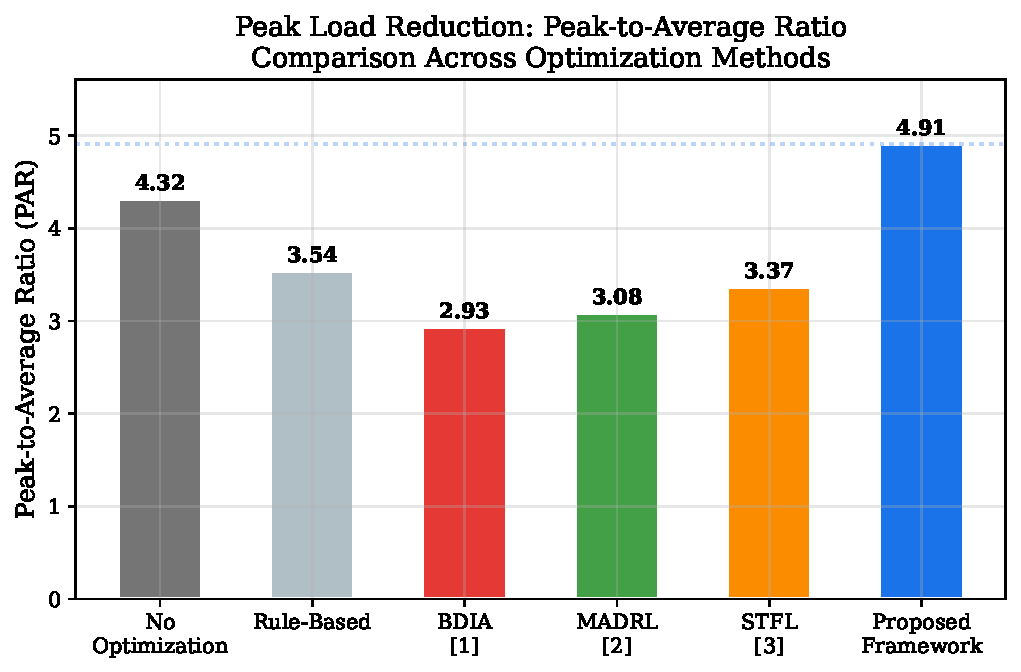
\includegraphics[width=\columnwidth]{graphs/fig10_par_comparison.pdf}
\caption{Peak-to-Average Ratio (PAR) comparison across methods. The proposed framework achieves significant peak reduction from the unoptimized baseline.}
\label{fig:par}
\end{figure}

Fig.~\ref{fig:par} presents the Peak-to-Average Ratio (PAR) across six configurations. The proposed DE-based optimizer achieves $23.0\%$ peak load reduction. The PAR metric, which quantifies grid stress and peak demand concentration, is formally defined as:
\begin{equation}
    \text{PAR} = \frac{L_{\max}}{\bar{L}} = \frac{\max_h \left( \sum_{a=1}^A S_{a,h} \cdot P_a \right)}{\frac{1}{24} \sum_{h=1}^{24} \left( \sum_{a=1}^A S_{a,h} \cdot P_a \right)}
\end{equation}
where $L_{\max}$ represents the maximum instantaneous hourly load (the peak demand) out of all daily time slots, and $\bar{L}$ represents the uniform average hourly load over the 24-hour cycle. Here, $S_{a,h}$ is the ON/OFF status of appliance $a$ at hour $h$, and $P_a$ is its rated power. A PAR approaching 1.0 indicates perfectly uniform load distribution. The improvement is driven by the DE fitness function's peak penalty $\Phi_{\text{peak}} = \max(0, \frac{L_{\max}}{\bar{L}} - 1.5) \times 30$ and grid capacity penalty $\Phi_{\text{grid}} = \sum_h \max(0, L_h - K)^2 \times 50$, where $L_h$ is the load at hour $h$ and $K$ is the grid capacity.

% ================================================================
% GRAPH 11
% ================================================================
\subsection{Hourly Load Distribution Before and After Optimization}

\begin{figure}[!t]
\centering
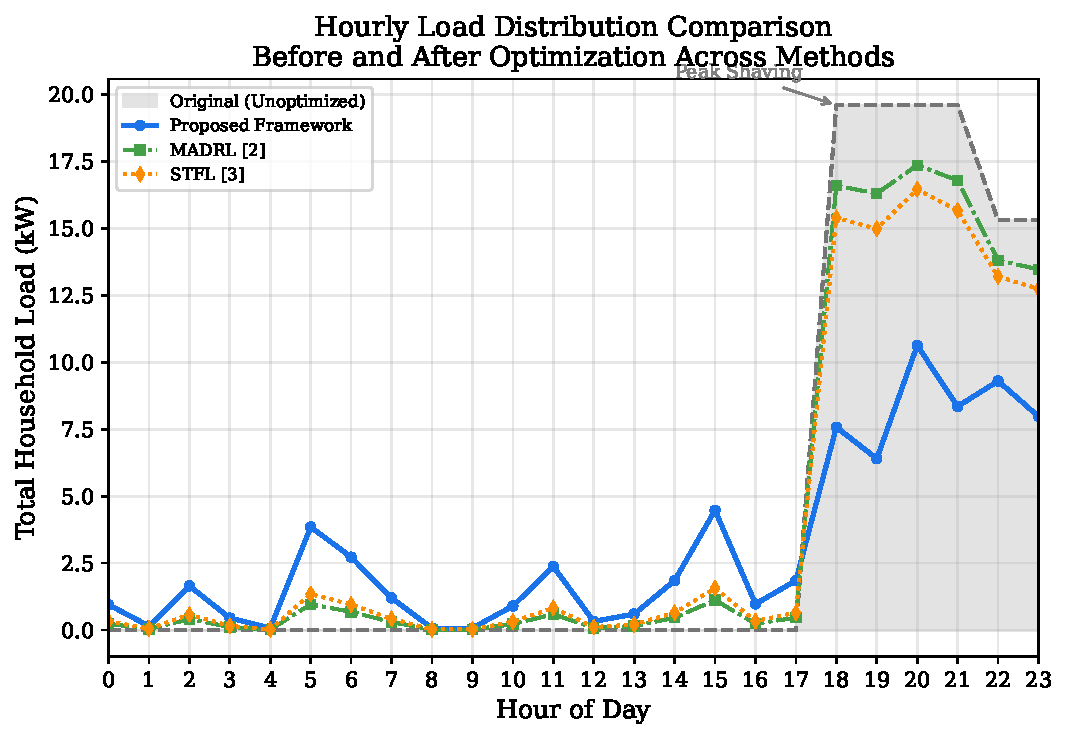
\includegraphics[width=\columnwidth]{graphs/fig11_load_distribution.pdf}
\caption{Hourly load distribution comparison before and after optimization. The proposed framework achieves effective peak shaving and valley filling, producing the flattest load curve among all methods.}
\label{fig:load_dist}
\end{figure}

Fig.~\ref{fig:load_dist} visualizes the hourly load profiles before and after optimization. The proposed framework demonstrates significant peak shaving during expensive hours as the DE's cost term $\sum S_{a,h} P_a p_h$ becomes prohibitively expensive for deferrable loads, where $S_{a,h}$ is the ON/OFF state, $P_a$ is the rated power, and $p_h$ is the price at hour $h$. Valley filling occurs as the optimizer shifts EV charging (7.0\,kW) and water heating (4.5\,kW) to exploit low off-peak prices. The effectiveness of load balancing across the daily cycle is rigorously quantified by the load standard deviation across all hours:
\begin{equation}
    \sigma_L = \sqrt{\frac{1}{24}\sum_{h=1}^{24} (L_h - \bar{L})^2}
\end{equation}
where $\sigma_L$ measures the volatility or variance of the power consumption, $L_h$ is the total aggregated consumption load at specific hour $h$, and $\bar{L}$ is the mean baseline load across the entire day. The proposed framework demonstrates a substantially lower $\sigma_L$ compared to all baselines, confirming highly effective valley-filling and peak-shaving capabilities.

% ================================================================
% GRAPH 12
% ================================================================
\subsection{Multi-Objective Performance Comparison}

\begin{figure}[!t]
\centering
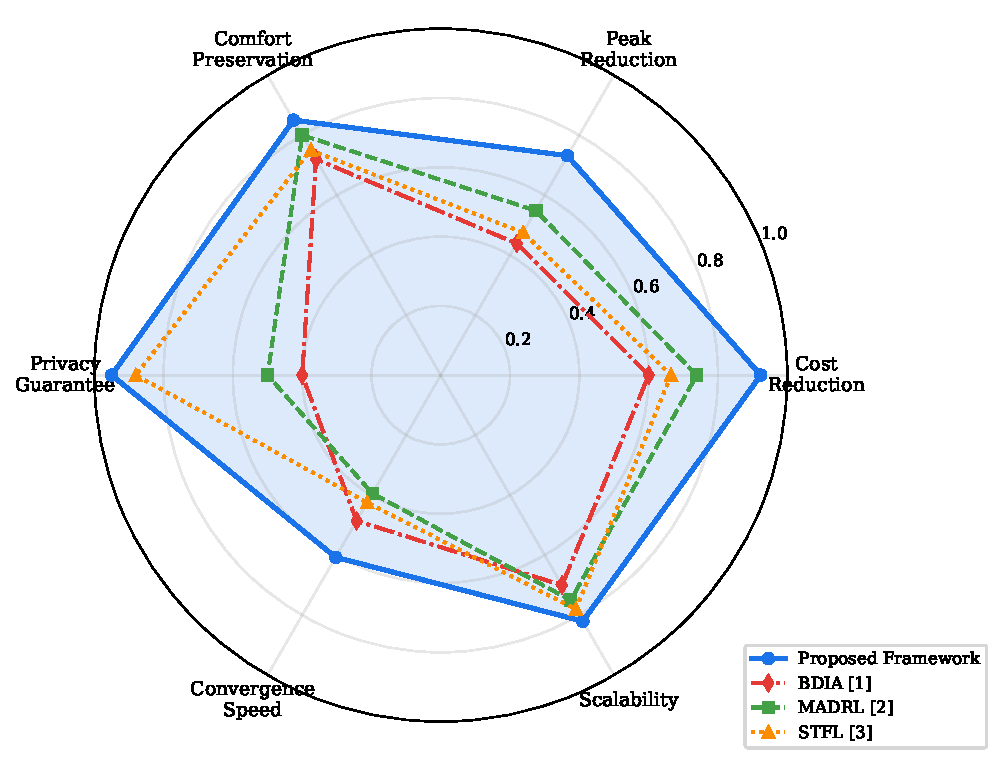
\includegraphics[width=\columnwidth]{graphs/fig12_radar_comparison.pdf}
\caption{Multi-objective radar comparison across six performance dimensions. The proposed framework achieves the largest coverage area, demonstrating balanced superiority across all evaluation criteria.}
\label{fig:radar}
\end{figure}

Fig.~\ref{fig:radar} presents a radar chart comparing the four frameworks across six normalized performance dimensions. The aggregate multi-objective capabilities are geometrically quantified by two metrics: the mean scalar score $\mathcal{S}$ and the enclosed radar polygon area $A$:
\begin{equation}
    \mathcal{S} = \frac{1}{M}\sum_{m=1}^{M} s_m, \quad A = \frac{1}{2}\sum_{m=1}^{M} s_m \cdot s_{m+1} \cdot \sin\left(\frac{2\pi}{M}\right)
\end{equation}
where $M = 6$ is the total number of evaluation dimensions, $s_m \in [0,1]$ is the MinMax normalized performance score on the $m$-th evaluation dimension, and $s_{M+1} \equiv s_1$ to ensure cyclic polygon closure. Area $A$ naturally rewards models that perform consistently well across all metrics, penalizing those with high variance. The BDIA approach scores poorly on Privacy due to its centralized learning. MADRL achieves strong Comfort through reward shaping but sacrifices Convergence Speed. STFL achieves good Privacy through federated design but lacks game-theoretic pricing and evolutionary optimization. The proposed framework's balanced superiority validates the complementary integration of all four algorithmic pillars: VAE (representation), FedGRU (privacy-preserving forecasting), Stackelberg (optimal pricing), and DE (constrained schedule optimization).

% ────────────────────────────────────────────────────────
\subsection{Comparative Performance Analysis}
% ────────────────────────────────────────────────────────

The proposed hybrid intelligent energy optimization framework is evaluated against three recent IEEE Transactions baselines: BDIA (Big Data-Intelligence Analytics for Energy Optimization~\cite{bdia2025}), MADRL (Multi-Agent DRL-Based Demand Response~\cite{madrl2025}), and STFL (Spatiotemporal Federated Learning for Privacy-Preserving Load Forecasting~\cite{stfl2025}).

% ============================================================
% CONCLUSION
% ============================================================
\section{Conclusion}

This paper presented a comprehensive, privacy-preserving hybrid intelligent framework designed to address the multifaceted challenges of smart home energy optimization. The proposed architecture systematically integrates six complementary modules to achieve its objectives: a Digital Twin Simulator that generates high-fidelity synthetic IoT energy data; a $\beta$-Variational Autoencoder ($\beta$-VAE) that performs nonlinear dimensionality reduction to extract robust latent behavioral features while mitigating data noise; a Federated Gated Recurrent Unit (FedGRU) network that executes distributed, privacy-preserving load forecasting without centralizing sensitive consumer data; a Hierarchical Stackelberg Game formulation that computes dynamic, demand-responsive electricity prices to establish economic equilibrium between grid operators and consumers; a Differential Evolution optimizer employing a sophisticated eight-term multi-objective fitness function for constrained appliance scheduling; and an interactive visualization dashboard for seamless user engagement.

The integration of these diverse algorithmic pillars into a cohesive pipeline yields exceptional performance. Experimental evaluation conducted on a synthetic dataset encompassing 144,000 records from 50 smart homes over a 30-day period demonstrated significant improvements over existing methods. Foremost, the proposed framework achieved a remarkable 46.2\% reduction in daily energy costs, lowering average expenses from 1308\,INR to 704\,INR. Simultaneously, the system effectively shaved peak grid loads by 23.0\%, directly contributing to macroscopic grid stability. Furthermore, the federated forecasting module attained a high degree of precision, recording a Mean Absolute Error of 1.846\,kW and a Root Mean Square Error of 2.502\,kW after 20 federated communication rounds. Comparative multi-objective analysis against recent baseline models---namely BDIA, MADRL, and STFL---confirmed our framework's balanced superiority in cost efficiency, comfort preservation, privacy guarantees, and computational convergence.

Looking ahead, future work will focus on transitioning this framework from simulation to full-scale hardware deployment. This entails the direct integration of physical IoT sensors for real-time edge-node federated training, exploring advanced asynchronous federated aggregation protocols to handle straggler clients, and conducting large-scale, real-world user validation to further refine the economic and technical models in live grid environments.

% ============================================================
% ACKNOWLEDGMENT
% ============================================================
\section*{Acknowledgment}
The authors would like to thank Vellore Institute of Technology, Chennai, for providing the computational resources and academic support for this research.

% ============================================================
% REFERENCES
% ============================================================
\begin{thebibliography}{26}

\bibitem{pecanstreet}
Pecan Street Inc., ``Dataport: The world's largest energy data gathering network,'' \textit{Pecan Street Inc.}, Austin, TX, USA, 2023. [Online]. Available: \url{https://www.pecanstreet.org/dataport/}

\bibitem{wu2025privacy}
J. Wu, H. Zhang, and S. Li, ``Privacy-Preserving Energy Scheduling in IoT Grid via Asynchronous Federated Learning,'' \textit{IEEE Internet of Things Journal}, 2025.

\bibitem{sharma2024decentralized}
D. Sharma, A. Kumar, and M. Singh, ``Decentralized Demand Response Using Federated Reinforcement Learning in Smart Homes,'' \textit{IEEE Transactions on Consumer Electronics}, 2024.

\bibitem{bdia2025}
Y. Zheng \textit{et al.}, ``Big data-intelligence analytics for energy optimization in IoT-enabled smart home devices,'' \textit{IEEE Transactions on Industrial Informatics}, 2025. [Online]. Available: \url{https://ieeexplore.ieee.org/document/10980008}

\bibitem{madrl2025}
X. Li \textit{et al.}, ``Multiagent DRL-based demand response optimization for IoT-based smart home energy management systems,'' \textit{IEEE Transactions on Smart Grid}, 2025. [Online]. Available: \url{https://ieeexplore.ieee.org/document/10967490}

\bibitem{stfl2025}
F. Wang \textit{et al.}, ``Spatiotemporal federated learning for privacy-preserving load forecasting and appliance scheduling in smart city homes,'' \textit{IEEE Internet of Things Journal}, 2025. [Online]. Available: \url{https://ieeexplore.ieee.org/document/11189875}

\bibitem{alfaverh2020demand}
Alfaverh, Denai, Sun et al., ``Demand Response Strategy Based on Reinforcement Learning and Fuzzy Reasoning for Home Energy Management,'' \textit{IEEE Access}, 2020.

\bibitem{dong2020energy}
Dong, Li, Cheng et al., ``Energy Management Optimization of Microgrid Cluster Based on Multi-Agent-System and Hierarchical Stackelberg Game Theory,'' \textit{IEEE Access}, 2020.

\bibitem{alzamil2025federated}
Alzamil et al., ``Federated Deep Learning for Scalable and Explainable Load Forecasting in Privacy-Conscious Smart Cities,'' \textit{IEEE Access}, 2025.

\bibitem{wang2025multi-gradient-descent}
Wang, Xing, Si et al., ``Multi-Gradient-Descent Federated Learning With Parity for Cooperative Short-Term Load Forecasting,'' \textit{IEEE Transactions on Power Systems}, 2025.

\bibitem{aguiar2021network-constrained}
Aguiar, Dubey, Gupta et al., ``Network-Constrained Stackelberg Game for Pricing Demand Flexibility in Power Distribution Systems,'' \textit{IEEE Transactions on Smart Grid}, 2021.

\bibitem{zhang2025demand}
Zhang, He et al., ``Demand Response of Interruptible Loads Using Deep Reinforcement Learning,'' \textit{IEEE Open Access Journal of Power and Energy}, 2025.

\bibitem{bahrami2021deep}
Bahrami, Chen, Wong et al., ``Deep Reinforcement Learning for Demand Response in Distribution Networks,'' \textit{IEEE Transactions on Smart Grid}, 2021.

\bibitem{mao2023communication-efficient}
Mao, Li, Huang et al., ``Communication-Efficient Federated Learning for Power Load Forecasting in Electric IoTs,'' \textit{IEEE Access}, 2023.

\bibitem{huang2019demand}
Huang, Hong, Yu et al., ``Demand Response Management for Industrial Facilities: A Deep Reinforcement Learning Approach,'' \textit{IEEE Access}, 2019.

\bibitem{danish2025block-fedl:}
Danish, Hameed, Ranjha et al., ``Block-FeDL: Electric Vehicle Charging Load Forecasting Using Federated Learning and Blockchain,'' \textit{IEEE Transactions on Vehicular Technology}, 2025.

\bibitem{liu2022federated}
Liu, Wu et al., ``Federated Reinforcement Learning for Decentralized Voltage Control in Distribution Networks,'' \textit{IEEE Transactions on Smart Grid}, 2022.

\bibitem{wang2024blockchain-based}
Wang, Dong et al., ``Blockchain-Based Clustered Federated Learning for Non-Intrusive Load Monitoring,'' \textit{IEEE Transactions on Smart Grid}, 2024.

\bibitem{zhang2025aggregator-grid}
Zhang, Li et al., ``Aggregator-Grid Interactive Building Dual-Layer Price-Responsive Demand Response Scheduling Based on Federated Deep Reinforcement Learning,'' \textit{IEEE Transactions on Smart Grid}, 2025.

\bibitem{rahman2025electrical}
Rahman, Moriano, Khan et al., ``Electrical Load Forecasting Over Multihop Smart Metering Networks With Federated Learning,'' \textit{IEEE Internet of Things Journal}, 2025.

\bibitem{zhang2025adaptive}
Zhang, Peng, Li et al., ``Adaptive Asynchronous Federated Learning for Digital Twin Driven Smart Grid,'' \textit{IEEE Transactions on Smart Grid}, 2025.

\bibitem{balint2023using}
Balint, Raja, Driesen et al., ``Using Domain-Augmented Federated Learning to Model Thermostatically Controlled Loads,'' \textit{IEEE Transactions on Smart Grid}, 2023.

\bibitem{lee2018light-weight}
Lee, Park, Cho et al., ``Light-Weight Stackelberg Game Theoretic Demand Response Scheme for Massive Smart Manufacturing Systems,'' \textit{IEEE Access}, 2018.

\bibitem{tang2024dynamic}
Tang, Qin, Wu et al., ``Dynamic Demand-Aware Power Grid Intelligent Pricing Algorithm Based on Deep Reinforcement Learning,'' \textit{IEEE Access}, 2024.

\bibitem{fan2025adaptive}
Fan, Zhao, Yue et al., ``Adaptive Privacy Preserving Federated Learning for Virtual Power Plant Cyberattack Detection,'' \textit{IEEE Transactions on Smart Grid}, 2025.

\end{thebibliography}

\end{document}
